\documentclass[11pt,a4paper,english]{article}
\usepackage[titletoc, title]{appendix}
\usepackage{amsmath}
\usepackage{amssymb}
\usepackage{bm}
\usepackage{array}
\usepackage{babel}
\usepackage{bbding}
\usepackage{color}
\usepackage[normal]{caption}
\usepackage{subcaption}
\usepackage{epsfig}
\usepackage{graphicx}
\usepackage{pdflscape}
\usepackage{lipsum}
\usepackage{psfrag}
\usepackage{proofapnd}
\usepackage[round]{natbib}
\usepackage[table,xcdraw]{xcolor}
\usepackage{afterpage}

%% Better roman enumeration list; no conflict with hyperref
\usepackage{enumerate}
\newenvironment{enumeroman} { %
\begin{enumerate}[(i)]
} { %
\end{enumerate}}%

\newenvironment{alphlist} { %
  \begin{enumerate}[(a)]
} { %
\end{enumerate}} %

\usepackage{rotating}
\usepackage[margin=2cm]{geometry} % for the same margin
\usepackage{latexsym}
\usepackage{float}
\usepackage{setspace}
\usepackage{slashbox}
\usepackage{enumitem}
\usepackage{multirow, tabularx,longtable, ragged2e, booktabs, siunitx}

\sisetup{output-decimal-marker = {.}}
\newcommand{\ra}[1]{\renewcommand{\arraystretch}{#1}}
\newcolumntype{Y}{>{\centering\arraybackslash}X}
\newcolumntype{C}{>{\Centering\arraybackslash}X}
\newcolumntype{s}{>{\hsize=.2\hsize \Centering\arraybackslash}X}

\usepackage{authblk}
\usepackage{hyperref}
\usepackage{indentfirst} 
\bibliographystyle{ecta}

\definecolor{markergreen}{rgb}{0.6, 1.0, 0}
\definecolor{darkgreen}{rgb}{0, .5, 0}
\definecolor{darkred}{rgb}{.7,0,0}
\definecolor{markergreen}{rgb}{0.6, 1.0, 0}
\definecolor{darkgreen}{rgb}{0, .5, 0}
\definecolor{darkorange}{rgb}{1,0.3,0}
\definecolor{darkred}{RGB}{.7,0,0}
\definecolor{darkblue}{RGB}{0,29,245}
\definecolor{orange}{RGB}{239, 133, 54}
\definecolor{lightblue}{RGB}{59, 188, 175}

\definecolor{plt1}{RGB}{31, 119, 180}
\definecolor{plt2}{RGB}{255, 127, 14}
\definecolor{plt3}{RGB}{44, 160, 44}
\definecolor{plt4}{RGB}{214, 39, 40}
\definecolor{plt5}{RGB}{148, 103, 189}
\definecolor{plt6}{RGB}{140, 86, 75}
\definecolor{plt7}{RGB}{227, 119, 194}
\definecolor{plt8}{RGB}{127, 127, 127}
\definecolor{plt9}{RGB}{188, 189, 34}
\definecolor{plt10}{RGB}{23, 190, 207}

\providecommand{\marker}[1]{\fcolorbox{markergreen}{markergreen}{{#1}}}
\providecommand{\mj}[1]{\textcolor{darkred}{#1}}
\providecommand{\francis}[1]{\textcolor{darkgreen}{#1}}
\providecommand{\natp}[1]{\textcolor{darkorange}{#1}}

\setlist[itemize]{leftmargin=*}
\setlist[description]{leftmargin=*}

\captionsetup{font={onehalfspacing,small}, labelfont=bf}

\title{\LARGE \bf Hedging Cryptos with Bitcoin Futures}
%\title{\natp{\large\bf Hedging Cryptocurrencies with Bitcoin Futures}}
\author{
	\begin{tabular}[t]{ccc}
		\and
        Francis Liu\thanks{
			Department of Business and Economics, Berlin School of Economics and Law, Badensche Str. 52, 10825 Berlin, Germany.
            Blockchain Research Center, Humboldt-Universität zu Berlin, Germany.
            International Research Training Group
1792, Humboldt-Universität zu Berlin, Germany.
     E-mail: \texttt{Francis.Liu@hwr-berlin.de}.}

		 \and
        Natalie Packham\thanks{
			Department of Business and Economics, Berlin School of Economics and Law, Badensche Str. 52, 10825 Berlin, Germany.
            International Research Training Group 1792, Humboldt-Universität zu Berlin, Germany.
     E-mail: \texttt{packham@hwr-berlin.de}.}

        \and
		Meng-Jou Lu
        \thanks{
             Department of Finance, Asia University, 500, Lioufeng Rd., Wufeng, Taichung 41354, Taiwan
             Department of Finance, Asia University, 500, Lioufeng Rd., Wufeng, Taichung 41354, Taiwan
     E-mail: \texttt{mangrou@gmail.com}.}

		 \and
         Wolfgang Karl H\"ardle\thanks{
			Blockchain Research Center, Humboldt-Universit\"at zu Berlin, Germany. Wang Yanan Institute for Studies in Economics, Xiamen University, China. Sim Kee Boon Institute for Financial Economics, Singapore Management University, Singapore. Faculty of Mathematics and Physics, Charles University, Czech Republic. National Yang Ming Chiao Tung University, Taiwan.
     E-mail: \texttt{haerdle@wiwi.hu-berlin.de}.}
        \thanks{ Financial support of the European Union's Horizon 2020 research and innovation program ``FIN-TECH: A Financial supervision and Technology compliance training programme" under the grant agreement No 825215 (Topic: ICT-35-2018, Type of action: CSA), the European Cooperation in Science \& Technology COST Action grant CA19130 - Fintech and Artificial Intelligence in Finance - Towards a transparent financial industry, the Deutsche Forschungsgemeinschaft's IRTG 1792 grant,
                 the Yushan Scholar Program of Taiwan %(\begin{CJK}{UTF8}{gbsn}\zh{台灣玉山學者計劃}\end{CJK}),
                 the Czech Science Foundation's grant no. 19-28231X / CAS: XDA 23020303, and DFG IRTG 1792 gratefully acknowledged.
     }
	\end{tabular}
}
\date{This version: \today}
%%%%%%%%%%%%%%%%%%%%%%%%%%%%%%%%%%%%%%%%%%%%%%%%%%%%%%%%%%%%%%%%%%%%%%%%%%%%%%%%%%%%%%%%%%%%%%%%
\renewcommand{\baselinestretch}{1.2}
%\newcommand{\indicator}{$1{\hskip -2.5 pt}\hbox{I}$}
\newcommand{\indicator}{I}
\input{definitions}

\begin{document}

\newtheorem{lemma}{Lemma}
\newtheorem {proposition}[lemma]{Proposition}
\newtheorem {corollary}{Corollary}
\newtheorem {theorem}{Theorem}
\newtheorem{claim}[lemma]{Claim}
\newtheorem{comment}[lemma]{Comment}
\newtheorem{example}[lemma]{Example}
\newtheorem{fact}[lemma]{Fact}
\newtheorem{defn}[lemma]{Definition}
\newtheorem{exercise}{Exercise}[section]

\newtheorem{programming}[exercise]{Programming assignment}
\newenvironment{proof}{{\flushleft\textbf{\textsl{Proof.\ \ }}}}{\hfill{\hfill\rule{2mm}{2mm}}}
\pagenumbering{arabic}

\maketitle

%%%%%%%%%%%%%%%%%%%%%%%%%%%%%%%%%%%%%%%%%%%%%%%%%%%%%%%%%%%%%%%%%%%%%%%%%%%%%%%%%%%%%%%%%%%%%%%
\begin{abstract}
  \footnotesize{

The introduction of derivatives on Bitcoin enables investors to hedge risk exposures in cryptocurrencies.
Because of volatility swings and jumps in cryptocurrency prices, the traditional variance-based approach to obtain hedge ratios may not be suitable for hedgers.
In this work, we consider two extensions of the traditional approach: first, different dependence structures are modelled by different copulae, such as the Gaussian, Student-t, Normal Inverse Gaussian and Archimedean copulae;
second, different risk measures, such as value-at-risk, expected shortfall and spectral risk measures are employed to find the optimal hedge ratio.
Extensive out-of-sample tests using the data from the time period December 2017 until May 2021 give insights in the practice of hedging various cryptos and crypto indices, including Bitcoin,  Ethereum, Cardano, the CRIX index and a number of
crypto-portfolios.
Evidence shows that BTC futures can effectively hedge BTC and BTC-involved indices. 
This promising result is consistent across different risk measures and
copulae except for the Frank copula.
On the other hand, we observe complex and diverse dependence
structures between non-BTC-related cryptocurrencies and the BTC futures. 
As a consequence, the hedge performance of non-BTC-related
cryptocurrencies is mixed and even suitable for some assets.

\noindent {\bf JEL classification: G11, G13}  \\ %G11 and G13 in QF

\noindent {\bf Keywords:} Cryptocurrencies, risk management, hedging,
copulas}
\pagestyle{empty}
\end{abstract}

\clearpage
%%%%%%%%%%%%%%%%%%%%%%%%%%%%%%%%%%%%%%%%%%%%%%%%%%%%%%%%%%%%%%%%%%%%%%%%%%%%%%%%%%%%%%%%%%%%%%%%%%%%%%%%%%%%%%%%%%%%%%%%%%%%%%%%%%%%%%%%%%%%%%%%%%%%%%
%%%%%%%%%%%%%%%%%%%%%%%%%%%%%%%%%%%%%%%%%%%%%%%%%%%%%%%%%%%%%%%%%%%%%%%%%%%%%%%%%%%%%%%%%%%%%%%%%%%%%%%%%%%%%%%%%%%%%%%%%%%%%%%%%%%%%%%%%%%%%%%%%%%%%%
\section{Introduction}\label{sec:introduction}
THe cryptocurrency (CC) market is a fast-growing market.
Since the first cryptocurrency Bitcoin (BTC) surfaced \citep{nakamoto2009}, 
many more CCs now available on the market.
In response to the rapid development of the CC market, the CME Group
launched exchange-traded BTC futures contracts in December
2017.
At the time of writing, the CME Bitcoin futures is one of a few crypto futures that is available on regulated exchange that offers
regulated crypto futures \footnote{We thank the referees for reminding the authors that Bakkt BTC futures are also available on regulated exchange.}. 
As per the CME report on 25th of Nov, 2022, the average daily volume and open interest of the CME BTC futures are
\$1,220M and \$1,357M respectively \footnote{Data from CME: \url{https://www.cmegroup.com/ftp/bitcoinfutures/Bitcoin_Futures_Liquidity_Report_20221202.pdf}}.
The CME BTC futures is an attractive instrument for institutional investors to participate in or manage their exposure in the crypto
market because it is fully regulated. 

As more individual and institutional investors are adding CCs and CC
derivatives to their portfolios, the need to understand
downside risks and find suitable ways to hedge against extreme risks
is created. 
Fom a risk management perspective, the roller-coaster ride
of crypto prices may create significant basis risk, even when using
simple hedges involving crypto portfolios and BTC futures. This
requires analysing the dependence structure of cryptos and
futures beyond linear correlation. 

In this paper, we examine hedges of crypto portfolios
with Bitcoin futures. Owing to the asymmetry of crypto returns as
well as the occurrence of extreme events, we consider different 
dependence structures via a variety of copula models. We then optimise
the hedge ratio using different risk measures. A similar study was
conducted by \citep{barbi2014copula} for equity and FX portfolios.
\citet{barbi2014copula}'s work is based on \citet{cherubini2011copula}
to derive the distribution of linear combinations of margins with
copulae describing the dependence structure. We slightly extend their
results and come up with a formula for the linear combination of
random variables for our purpose.

The hedge ratio is the appropriate amount of futures contracts to hold
in order to eliminate the risk exposure in the underlying security.   
The determination of the hedge ratio relies primarily
on the dependence between BTC and futures prices.

Financial asset returns have long known to be non-Gaussian, see e.g.\
\citep{fama1963mandelbrot,Cont2001}. Specifically, Gaussian models
cannot produce the heavy tails and the asymmetry observed in 
asset returns, which in turn implies a consistent underestimation of
financial risks. 

Therefore, to minimize downside risk, one cannot solely rely on
second-order moment calculations. Moreover, variance as a risk measure
does not account for the variety of investors' utility functions. In
particular, it is known that  
investors are tail-risk averse, see \cite{menezes1980increasing}.
Copulae provide the flexibility to model multivariate random variables
separately by their margins and dependence structure.
The concept of copulae was originally developed (but not under this
name) by Wassily Hoeffding \citep{hoeffding1940masstabinvariante}
and later popularised by the work of Abe Sklar \citep{Sklar1959}.

Different risk measures account for investors' risk attitudes.
They serve as loss functions in the search process of the optimal
hedge ratio. Of the vast literature discussing the relationship between
risk measures and investors' risk attitudes, we refer readers to
\citet{artzner1999coherent} for an axiomatic 
approach of risk measure construction;
\citet{embrechts2002correlation} for reasoning of using expected
shortfall (ES) and spectral risk measures (SRM) in addition to
value-at-risk (VaR);
\citet{Acerbi2002} for direct linkages between risk measures and
investor's risk attitudes using the concept of a ``risk aversion
function''. 


In order to capture a variety of risk preferences, in addition to
variance, we include the risk measures value-at-risk (VaR), expected
shortfall (ES), and spectral risk measures (SRM). 
%Coherency is a very natural property that suggest diversification will reduce risk.
VaR is widely used by the finance industry and easy to understand. 
ES and SRM are chosen because of their coherence property, in
particular, they recognize diversification benefits.
SRM can also be directly related to an individual's utility function.
Examples are the exponential SRM and power SRM introduced by
\citet{dowd2008spectral}. 

Evaluating the hedging effectiveness of crypto derivatives has been done by many researchers. 
\citet{deng2020minimum} show that the crypto inverse futures is able to be used to hedge against BTC exposure.
\citet{alexander2020bitmex} crypto derivatives on BitMEX not only play an important role in price discovery of BTC,
 they can be used as hedging instrument to offset the movement of BTC price. 
\citet{sebastiao2020bitcoin} present promising results of using BTC futures to hedge BTC and other CCs. 
\citet{alexander2021hedging} extend the analysis to include the present of liquidation procedure in crypto exchanges. 
They show that hedgers are able to manage the liquidation probability while keeping a reasonable hedging capability from crypto derivatives. 

In this work, we study the effectiveness of hedging various CCs and
CC indices using the CME BTC futures under copula models and different
risk preferences. 
Through an extensive backtest,\footnote{We thank the data provider
  Tiingo (\href{https://www.tiingo.com/}{https://www.tiingo.com/}) for
  providing the crypto price data.}
 we find the ability of the CME BTC futures to hedge BTC and BTC-related
 indices promising, regardless of the choice of the copula (with the
 exception of the Frank copula) and risk measure. 
On the other hand, the ability of the CME BTC futures to hedge other CCs and CC indices
is affected by idiosyncratic factors such as regulatory factors and operational risk,
but the overall hedging effectiveness to other cryptos and crypto indices is far lower
than that to BTC.
We discuss the characteristics of the hedged portfolios constructed by range of risk measures-copulae pairs.

The paper is organized as follows. Section \ref{sec:optimal-hedge-ratio} introduces the notion of
an optimal hedge ratio as well as the backtest procedure deployed in this work;
Section \ref{sec:crm} presents the copulae used in this work as well as the calibration procedure;
Section \ref{subsec:spectral-risk-measures} provides the risk measures;
Section \ref{sec:results} discusses the backtest results; Finally,
Section 5 concludes the findings. 
All calculations in this work can be reproduced with the data and code
available at \href{http://www.quantlet.com/}{www.quantlet.com
  {\includegraphics[height=\baselineskip]{_pics/qletlogo_tr.png}}}. 
%%%%%%%%%%%%%%%%%%%%%%%%%%%%%%%%%%%%%%%%%%%%%%%%%%%%%%%%%%%%%%%%%%%%%%%%%%%%%%

\section{Optimal hedge ratio}\label{sec:optimal-hedge-ratio}

\subsection{Distribution of hedge portfolio}\label{subsec:DHP}
We form a portfolio with two assets, consisting of one unit in the
spot asset and a short position of $h$ units of a futures contract,
for example one Bitcoin and a short position in a CME Bitcoin
futures contract. 
The objective is to minimize the risk of the exposure in the spot. 
Let $R^S$ and $R^F$ be the (discrete) returns of the spot and
futures price. The (discrete) return of the portfolio is\footnote{%
In practice, as the nominal investment in the futures is zero, $R^F$
is understood as the return on the notional amount underlying the
futures contract. In other words, if both the spot price $S_{t-1}$
and the futures price $F_{t-1}$ are 
normalised to $1$, then the portfolio return will be identical to the
portfolio value change $\Delta V = \Delta S - h \Delta F$, where $\Delta S =
S_t-S_{t-1}$, etc.}
\begin{equation*}
R^h = R^S -h R^F.
\end{equation*}
%\natp{\em [I fixed this, please check.] [We need to discuss the
%  footnote. Generally, the portfolio return is $R_p = \sum_{i=1}^n w_i
%  R_i$. With the futures contract, the notional investment in the
%  futures is zero, so the portfolio return is $(S_0 (1+R^S) -h F_0
%  R^F)/S_0-1 = R^S-h R^F$, if $S_0=F_0$.]}

The risk of the hedged portfolio is measured by risk measure functions $\rho$s.
For example, a widely used risk measure is value-at-risk (VaR), which,
at the confidence level $\alpha$,
is derived from the $1-\alpha$ quantile of the return distribution. %  at the confidence level $\alpha$ is
% the absolute value of the $1-\alpha$-quantile of $R^h$, i.e., $\text{VaR}_{1-\alpha} =
% -F_{R^h}^{(-1)}(1-\alpha) = -\inf\{x \in \mathbb{R}: 1-\alpha \leq
% F_{R^h}(x) \}$, where $F_{R^h}$ is the distribution function of
% $R^h$.

If the portfolio is intended to reduce the risk of the spot position, then
we call this a hedged portfolio.
An optimal hedge ratio $h^*$ is a parameter that
minimizes the risk of the aforementioned portfolio
\begin{equation*}
h^* = \argmin_h \rho(R^h).
\end{equation*}

Obviously the cdf and pdf of $R^h$ and the risk measure depend on the
joint distribution of $R^S$ and $-hR^F$. However, optimising $h$
according to the joint pdf is unfavourable since one would need to
calibrate it whenever she updates $h$.
Another problem of using the joint pdf is that one lacks the
flexibility to model the margins separately from the dependence
structure. Copulae allow to overcome both of these problems. 

The advantage of using copulae is two-fold.
First, copulae are invariant under strictly
monotone increasing function \citep{schweizer1981nonparametric}, a
property used in Lemma \ref{lemma:copula} below. 
Second, copulae allow us to model the margins and dependence structure 
separately, a result known as Sklar's Theorem \citep{Sklar1959}, which
is given as Theorem \ref{theorem:sklar} below. 
See also \citep{Nelsen1999, joe1997multivariate, McNeil2005} for
Sklar's Theorem and more properties of copulae.

We adapt the definition of a two-dimensional copula from
\citep{Nelsen1999} as follows.

\begin{defi} [Bivariate copula]
  A {\em bivariate copula} is a function $C: [0,1]^2 \mapsto [0,1]$ with following properties:
  \begin{enumerate}
    \item For every $u,v$ in $[0,1]$,
      \[C(u,0)= C(0,v)=0, \]
    \[C(u,1)= u \text{, and}\]
    \[C(1,v)= v;\]
    \item For every $u_1,u_2, v_1, v_2$ in $[0,1]$ such that $u_1 \leq u_2$ and $v_1 \leq v_2$,
    \[C(u_2,v_2)-C(u_2,v_1)-C(u_1, v_2)+C(u_1,v_1) \geq 0.\]
  \end{enumerate}
  \end{defi}

The second property is called 2-non-decreasing.
In other words, a two-dimensional copula is the joint cdf of a two-dimensional random vector
on a unit square with uniform marginals.

The following Theorem, usually known as the Sklar's
Theorem, ensures the existence of copula which “couples” a 
joint distribution function to its univariate margins \citep[Theorem 2.3.3.]{Nelsen1999}.

% \natp{\em [This is not
%   correct. Copulas, as defined above, exist. Sklar's Theorem links
%   copulas to arbitrary joint distributions.]}

\begin{theorem}[Hoeffding-Sklar-Theorem]
  \label{theorem:sklar}
  Let $F$ be a joint distribution function with marginal distributions
  $F_X$ and $F_Y$. Then, there exists a copula $C:[0,1]^2 \mapsto
  [0,1]$ such that, for all $x,y\in \R$,
  \begin{equation}
    \label{eq:4}
    F(x,y)=C\{F_X(x), F_Y(y)\}.
  \end{equation}
  If the margins are continuous, then $C$ is unique; otherwise $C$ is
  unique on the range of the margins.

  Conversely, if $C$ is a copula and $F_X, F_Y$ are univariate
  distribution functions, then the function $F$ defined by (\ref{eq:4})
  is a joint distribution function with margins $F_X, F_Y$.
\end{theorem}

Hence, copula enables hedgers to model the dependence structure between the spot and futures separately from their marginals 
without any restriction imposed by the model assumption marginals.
For example, the marginals of multivariate Gaussian are always Gaussian, but marginals of copula can be any univariate marginals that hedgers favour. 
Since we want to focus on the effects of how dependence structure shapes hedging effectiveness, copula allows us to
make minimal model assumption on the marginals by deploying kernel density estimators with different bandwidths for the spot and futures. 

Regarding the theory behind copula, many basic results can be traced back to early
works of Wassily Hoeffding \citep{hoedffding1940, hoedffding1941}. 
The two works aim to derive a measure of relationship of variables which is invariant under change of scale. 
See also \citet{hoeffding2012collected} for English translations of
the original papers written in German. 

Another feature of copula that is important for hedgers is shown below. 

\begin{lemma}
  \label{lemma:copula}
  Let $h>0$ and let $X$ and $Y$ be continuous random variables. Then,
  the joint distribution of the portfolio positions 
  can be expressed via the joint distribution of the securities as
  follows:
  \begin{align}
  C_{X, hY}\left(F_X(s),F_{hY}(t)\right) = C_{X,
    Y}\left(F_X(s),F_{Y}(t/h)\right), \quad s,t\in \R.
    \end{align}
  \end{lemma}

\begin{proof}
  Since copulae are invariant under strictly monotone increasing
  function \citet[Theorem 3 (i)]{schweizer1981nonparametric} or
  \citet[Theorem 2.4.3]{Nelsen1999}, 
  \begin{equation*}
    C_{X, hY}\left(F_X(s),F_{hY}(t)\right) = C_{X, Y}\left(F_X(s),F_{hY}(t)\right).
    \end{equation*}
Re-writing the second argument of the copula gives
\begin{equation*}
  F_{hY}(t) = \mathbb{P}(hY \leq t)
  = \mathbb{P}(Y \leq t/h)
  = F_Y(t/h).
\end{equation*}
\end{proof}

Lemma \ref{lemma:copula} describes the fact that copula is invariance under linear transformation.
That means rescaling one random variable does not change the dependence structure captured by copula. 
Searching of optimal hedge ratio (numerically) requires frequent updates of the size $h$,
but with copula, the search does not require any recalibration.
Taking advantage of Lemma \ref{lemma:copula}, \citet{barbi2014copula}
introduce the distribution of linear combinations of random variables
using copulae. 
We slightly edit Corollary 2.1 of their work and yield the 
following correct expression of the distribution. 

\begin{proposition}
  \label{prop:dfrh}
  Let $X$ and $Y$ be two real-valued continuous random
  variables on a
  probability space $(\Omega, \F, \p)$ with
  absolutely continuous copula $C_{X, Y}$ and marginal distribution functions $F_{X}$
  and $F_{Y}$. Then, the distribution function of $Z=X-hY$, $h >0$,  is given by
  \begin{equation}
    \label{eq:3}
    F_{Z}(z) = 1- \int^1_0 D_1 C_{X, Y}
    \left[ u, F_{Y} \left\{ \frac{F^{(-1)}_{X}(u)-z}{h} \right\}
    \right]\, d u,   
  \end{equation}
  where, $F^{(-1)}$ denotes the inverse of $F$, i.e., the quantile
function.
\end{proposition}
Here, $D_1 C(u,v)=\displaystyle \frac{\partial}{\partial u}
C(u,v)$ and, see e.g.\ Equation (5.15) of \citet{McNeil2005},
\begin{equation}
  \label{eq:1}
  D_1 C_{X,Y}\{F_X(x), F_Y(y)\} = \p(Y\leq y|X=x).
\end{equation}
\begin{proof}
  Using the identity (\ref{eq:1}) gives
  \begin{align*}
    F_{Z}(z) &= \p(X - h Y\leq z) %
                 = \E\left\{\p\left(Y\geq \frac{X-z}{h}\Big|
                 X\right)\right\}\\[10pt]
               &= 1-\E\left\{\p\left(Y\leq \frac{X-z}{h}\Big|
                 X\right)\right\}% \\[10pt]
               = 1- \int_0^1 D_1 C_{X, Y}\left[u,
                 F_{Y}\left\{\frac{F^{(-1)}_{X}(u) -
                 z}{h}\right\}\right]\, d u.
  \end{align*}
  \end{proof}

\begin{corollary} The pdf of $Z$ can be written as
  \begin{align}
  f_{Z}(z) &= h^{-1}\int_0^1 c_{X, Y} \left[
  F_{Y}\left\{\frac{F^{(-1)}_{X}(u)-z}{h}\right\}, u
  \right]
   \cdot
  f_{Y}
  \left\{\frac{F^{(-1)}_{X}(u)-z}{h}\right\} du, \label{eq:density1}
  \end{align}
  \end{corollary}
Note that the pdf of $Z$ in the above proposition can be assessed via numerical integration
as long as we have the copula density and the marginal
densities.
A multivariate generalisation of the expression above and its proof can be found in Appendix \ref{sec:appendix}.

\subsection{Backtesting Procedure}\label{sec:empirical-procedure}
Time series of out-of-sample hedged portfolio returns that represent a hedger's profit and loss are obtained via the following steps.
We start from the earliest 300 data points of each spot-futures pair as training data:
\begin{enumerate}
\item \textbf{Construct univariate kernel density function (KDE)}:
  Construct the spot and futures' univariate kernel density functions separately
  using the Gaussian kernel. The bandwidths are determined separately by the refined plug-in method \citep[Section
  3.3.3]{hardle2004nonparametric}.
\item \textbf{Calibrate copulae}:
  Calibrate the copulae outlined in Section \ref{sec:crm} by the
  method of moments described in Section \ref{sec:estimation}.
\item \textbf{Select copula}:
  Compute the Akaike Information Criterion (AIC). The copula with the
  best (i.e. lowest) AIC is used for the next step. 
  A discussion of this step is found in Section \ref{subsec:copula-selection}.
\item \textbf{Determine optimal hedge ratio}:
  Determine the optimal hedge ratios with respect to different
  risk measures numerically. 
  To do so, we draw samples from the calibrated copulae and KDEs 
  and search for the hedge ratio that gives the lowest risk measure. 
  The risk measures are outlined in Section \ref{subsec:spectral-risk-measures}.
  The minimisation algorithm \textit{scipy.optimize.minimize} from the Python package {\em Scipy} \citep{2020SciPy-NMeth} is used for the search of optimal hedge ratio.
\item \textbf{Obtain out-of-sample hedged portfolio returns}: Apply the optimal hedge ratio to the test data to obtain out-of-sample hedged portfolio returns.
      The test data is the 5 data points subsequent to the last training data point. 
\item \textbf{Roll forward}: We roll forward by 5 data points and repeat the steps above until the test data reaches the end of the dataset.
\end{enumerate}

The collection of out-of-sample portfolio returns forms a non-overlapping time series since the step size is equal to test data length.
The time series represents the profit and loss if hedgers recalibrate copulae and adjust the hedge ratio every 5 days from the start to the end of the out-of-sample data period.
An intraday setup and its results are documented in Appendix \ref{sec:intraday}. 

The backtesting procedure without the copula selection step (step 3) is also carried out to examine the effects of deploying different copula. 
Section \ref{subsec:HP1} discusses the effects. 

\section{Copulae}\label{sec:crm}
To capture different aspects of the dependence structure between spot and futures, we consider
a range of different copulae. 
The copulae are the Gaussian-, $t$-, Frank-,
Gumbel-, Clayton-, mixture, NIG factor, and Plackett-copula. 
Figure~\ref{fig:copulaeScatterPlot} shows scatter plots of random
samples drawn from the copulae. 
\begin{figure}[t]
    \centering
  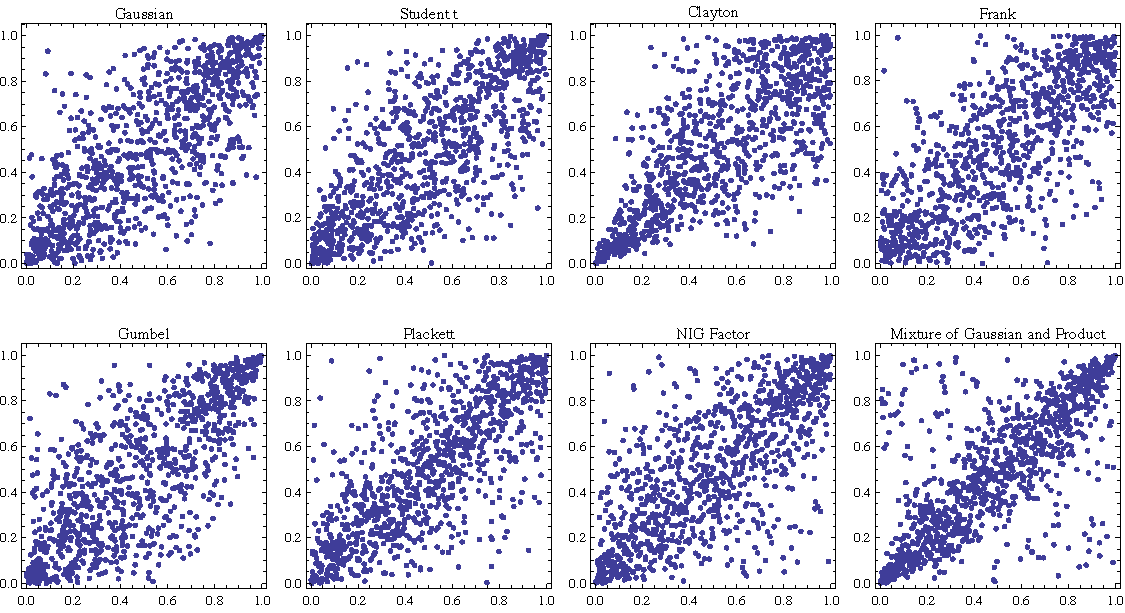
\includegraphics[width=\textwidth]{_pics/copulas_scatterplots.pdf}
  \caption{Scatterplots of samples drawn from various copulae. All
    copulae are calibrated to Spearman's $\rho$ of 0.75 before
    sampling.}\label{fig:copulaeScatterPlot} 
\end{figure}

As this hedging exercise concerns only portfolios with two assets, we
focus on the bivariate version of each copula. 

\subsection{Gaussian and $t$ Copulae}\label{sec:ellpitical-copulae}

The Gaussian and $t$ copulae are derived from Gaussian and $t$
distributions. 
The bivariate Gaussian copula is defined as
\begin{align*}
  \bm{C}(u,v) &= \Phi_{2, \rho}\{\Phi^{(-1)}(u), \Phi^{(-1)}(v)\} \nonumber \\
              &= \int_{-\infty}^{\Phi^{(-1)}(u)}
                \int_{-\infty}^{\Phi^{(-1)}(v)}
                \frac{1}{2\pi\sqrt{1-\rho^2}}
                \exp{\left\{
                \frac{s^2-2\rho st+t^2}{2(1-\rho^2)}
                \right\}} \dd s\, \dd t,\quad, u,v\in [0,1],
\end{align*}
where $\Phi_{2, \rho}$ is the bivariate Normal cdf
with zero mean, unit variance, with correlation coefficient $\rho$, and
$\Phi^{(-1)}$ is the quantile function of the univariate standard normal
distribution.
The Gaussian copula is fully specified by the correlation parameter $\rho$. \footnote{
The symbol $\rho$ is used to denote both the correlation parameter as
well as a general risk measure. However, it will be clear from the
context, what $\rho$ refers to.}
It has no tail dependence, which, in a finance context, implies that
it often underestimates tail risk.  

Kendall's tau $\tau_K$ and Spearman's rho $\rho_S$ of the bivariate Gaussian copula are
    \begin{equation*}
        \tau_K(\rho) = \frac{2}{\pi}\arcsin\rho, \quad\quad
        \rho_S(\rho) = \frac{6}{\pi}\arcsin\frac{\rho}{2}.
        \end{equation*}

The $t$-copula has the form
\begin{multline*}
        \bm{C}(u,v) = \bm{T}_{2, \rho, \nu}\{T^{(-1)}_\nu(u), T^{(-1)}_\nu(v)\}\\
        = \int_{-\infty}^{T^{(-1)}_\nu(u)}
               \int_{-\infty}^{T^{(-1)}_\nu(v)}
            \frac{\Gamma\left(\frac{\nu+2}{2}\right)}
            {\Gamma\left(\frac{\nu}{2}\right)\pi\nu\sqrt{1-\rho^2}}
             \left(
        1+\frac{s^2-2st\rho+t^2}{\nu}
        \right)^{-\frac{\nu+2}{2}}\, \dd s\, \dd t,
    \end{multline*}
where $\bm{T}_{2, \rho, \nu}$ denotes the 
bivariate $t$ cdf with dependence parameter $\rho$ and degrees of
freedom parameter $\nu$, $\nu>2$,
and where $T^{(-1)}_\nu(\cdot)$ is the quantile function of a standard
$t$ distribution with parameter $\nu$. 

The $t$-copula and Gaussian copula with parameter $\rho$ have equal $\tau_K$s, \citep[see][and references therein]{demarta2005t}.
The $t$-copula has non-zero upper and lower tail dependence, which makes it more appropriate for dependence modelling in finance than the Gaussian copula.

\subsection{Archimedean copulae}\label{sec:archimedean-copula}
The family of Archimedean copulae forms a large class of copulae with
many convenient features.

Archimedean copulas are determined via a simple parametric form of the
dependence structure. A prominent feature is the ability to model
asymmetric dependence structures.  

In general, an Archimedean copula takes the form
\begin{align*}
  \bm{C}_\theta(u,v) = \psi^{(-1)}\{\psi(u; \theta), \psi(v; \theta); \theta\},\quad u,v\in [0,1],
    \end{align*}
where $\psi:[0,1] \rightarrow [0,\infty)$ is a continuous, strictly
decreasing and convex function such that $\psi(1)=0$ for any
permissible dependence parameter $\theta$. The function $\psi$ is 
called the generator, with $\psi^{(-1)}$ its inverse.

The {\em Frank copula\/} (B3 in \citet{joe1997multivariate}) takes the form
\begin{align*}
    \bm{C}_{\theta}(u,v) &= \frac{1}{\theta}
    \log \left\{
    1 + \frac{(e^{-\theta u}-1)(e^{-\theta v}-1)}{e^{-\theta}-1}
    \right\}, \quad u,v\in [0,1],
    \end{align*}
    with $\theta \in [0, \infty]$ the dependence parameter. 
    It is a symmetric copula and cannot produce any tail
    dependence. The following parameters correspond perfect dependence
    and independence: $\bm{C}_{-\infty} = \bm{M}$, $\bm{C}_1 = \bm{\Pi}$,
    and $\bm{C}_\infty = \bm{W}$. 
    The Frank copula has $\tau_K$ :
\begin{align*}
    \tau_K(\theta) = 1-4\frac{D_1\{-\log(\theta)\}}{\log(\theta)},
    \end{align*}

where $D_1$ and $D_2$ are the Debye function of order 1 and 2, with
the Debye function defined as $D_n =
\frac{n}{x^n}\int_0^x\frac{t^n}{e^t-1}dt$.
We refer readers to \citet[p.998]{abramowitz1972handbook} for definition of the Debye function. 

The {\em Gumbel copula\/} (B6 in \citet{joe1997multivariate}) has
distribution function
\begin{equation*}
  \bm{C}_{\theta}(u,v) = \exp{-\{ (-\log(u))^\theta +(-\log(v))^\theta 
    \}^{\frac{1}{\theta}}},
\end{equation*}
where $\theta \in [1,\infty)$ is the dependence parameter.
Its  Kendall's tau takes the form \begin{equation*}
  \tau_K(\theta) =\frac{\theta-1}{\theta}. 
 \end{equation*}
It has upper tail dependence with dependence parameter $\lambda^U
= 2-2^{\frac{1}{\theta}}$ and displays no lower tail dependence. 
    
While the Gumbel copula cannot model perfect counter-dependence
\citep{Nelsen2002}, $\bm{C}_{1} = \bm{\Pi}$ models independence, 
and $\lim_{\theta\rightarrow\infty} \bm{C}_\theta = \bm{W}$ models
perfect dependence. 


The {\em Clayton copula\/} takes the form
\begin{equation*}
  \bm{C}_{\theta}(u,v) = \left\{
    \max(u^{-\theta}+v^{-\theta}-1,0)\right\}^{-\frac{1}{\theta}},
\end{equation*}
where $\theta \in (-\infty, \infty)$ is the dependence parameter.
The Clayton copula, by contrast to Gumbel copula,
generates lower tail dependence with $\lambda^L =
2^{-\frac{1}{\theta}}$, but cannot generate upper tail dependence.
Moreover, $\lim_{\theta\rightarrow -\infty} \bm{C}_\theta = \bm{M}$, $\bm{C}_0 =
\bm{\Pi}$, and $\lim_{\theta\rightarrow\infty} \bm{C}_\theta = \bm{W}$. 
The Kendall's tau of the Clayton copula is given by 
\begin{align*}
    \tau_K(\theta) =\frac{\theta}{\theta+2}.
    \end{align*}

\subsection{Mixture Copula}\label{sec:mixture-copula}
The mixture copula is a linear combination of copulae. 
The distribution of a 2-dimensional random variable
$\bm{X}=(X_1,X_2)^\top$ is written as linear combination of $K$
copulae 
\begin{equation*} 
    \bm{C}(u,v)= \sum_{k=1}^K p^{(k)} \cdot \bm{C}^{(k)}\{F^{(-1)}_{X_1}(u),
    F^{(-1)}_{X_2}(v); \bm{\theta^{(k)}}\}, \quad u,v\in [0,1].
  \end{equation*}
  Here, $\bm{\theta^{(k)}}$ refers to the parameters of the
    $k$-th copula.
   
While Kendall's tau of the mixture copula is not known in closed form,
Spearman's rho is easily derived as 
\begin{equation*}
  \rho_S = \sum_{k=1}^K p^{(k)} \cdot \rho_S^{(k)}. 
\end{equation*}

An example of a mixture copula is the Fr\'echet class of copulae, which
are given by convex combinations of $\bm{W}$, $\bm{\Pi}$, and $\bm{M}$
\citep{Nelsen1999}.  

We use the {\em Gaussian Mix Independent Copula (GMI)} in our analysis,
i.e., 
\begin{equation*}
  \bm{C}(u,v) = p\, \bm{C}^\text{Gaussian}_\theta (u,v) + (1-p)(uv),\quad p\in [0,1].
\end{equation*}

This mixture models the amount of ``random noise'' that appears in the
off-diagonal region of the dependence structure where the Gaussian copula has no control.
In the hedging exercise, the structure of the off-diagonal ``random noise'' is not our main concern, 
but the amount of it might affect the hedging effectiveness.

\subsection{NIG factor copula}

Normal Inverse Gaussian (NIG) distribution is a flexible and yet analytical tractable distribution introduced by
\citep{BarndorffNielsen1997}.
The {\em NIG factor copula} is constructed based on the characteristics of the NIG disribution. 
This section presents the version of NIG factor copula we use in this work.
The NIG distribution has density function
\begin{equation*}
  g(x; \alpha,\beta, \mu, \delta) = \frac{\alpha}{\pi} \e^{\delta
    \sqrt{\alpha^2-\beta^2} -\beta\mu} \frac{1}{q((x-\mu)/\delta)}
  K_1\left[\delta \alpha q\left(\frac{x-\mu}{\delta}\right) \right]
  \e^{\beta x},\quad x>0,
\end{equation*}
where $q(x) = \sqrt{1+x^2}$ and where $K_1$ is the modified Bessel
function of third order and index $1$. The parameters satisfy $0\leq
|\beta|\leq \alpha$, $\mu\in \R$ and $\delta>0$, and have
the following interpretation: $\mu$ and $\delta$ are location and
scale parameters, respectively, $\alpha$ determines the heaviness of
the tails and $\beta$ determines the degree of asymmetry. If
$\beta=0$, then the distribution is symmetric around $\mu$.

The cdf and quantile function of NIG distribution, denoted by $G(x; \alpha, \beta, \mu, \delta)$ and $G^{(-1)}(x; \alpha, \beta, \mu, \delta)$,
 have no known analytical form.
 In this work, they are computed via numerical integration of the density and by simulation.

The NIG distribution belongs to
the class of so-called {\em normal
variance-mean mixture distributions},  (see Section 3.2 of 
\citet{McNeil2005}): $X$ follows an
$\text{NIG}(\alpha,\beta,\mu,\delta)$ distribution if $X$ conditional
on $W$ follows a normal distribution with mean $\mu+\beta W$ and
variance $W$, i.e., 
\begin{equation*}
  X|W\stackrel{\mathcal L}\sim \Ncdf(\mu + \beta W, W),
\end{equation*}
where $W$ follows an {\em inverse Gaussian distribution}, denoted by
$\text{IG}(\delta, \sqrt{\alpha^2-\beta^2})$.

The simulation procedure of the NIG$(\alpha, \beta, \mu, \delta)$
distribution is a natural result of the above decomposition.  
To simulate the NIG distribution, first simulate a random variable $w \sim IG(\delta, \sqrt{\alpha^2-\beta^2})$, 
then simulate $x \sim N(\mu+ \beta w, w|w)$. 

The moment-generating function of the NIG distribution is given by
\begin{equation*}
  M(u; \alpha, \beta, \mu, \delta) = \exp\left( \delta
    \left(\sqrt{\alpha^2-\beta^2} - \sqrt{\alpha^2 - (\beta +
        u)^2}\right) + \mu u\right). 
\end{equation*}
As a direct consequence, moments are easily calculated with the
expectation and variance of the NIG distribution being
\begin{align*}
  \mathbb E X &= \mu +
                \frac{\delta \beta}{\sqrt{\alpha^2-\beta^2}}
  \end{align*}
\begin{align} \label{eq:5}
  \text{Var}(X) &= \frac{\alpha^2\delta}{(\alpha^2-\beta^2)^{3/2}}.
\end{align}

It is easily seen from the moment-generating function that the NIG distribution is preserved under linear combinations, provided
the variables share the parameters $\alpha$ and $\beta$. 
\begin{prop}
  \label{prop:NIG}
  Let $Z\sim \text{NIG}(\alpha, \beta, \mu, \delta)$ and
  $Z_i\sim \text{NIG}(\alpha, \beta, \mu_i, \delta_i)$,
  $i=1,\ldots, n$ be independent NIG-distributed random
  variables. Then:
  \begin{enumerate}
  \item  $X_i = Z + Z_i\sim \text{NIG}(\alpha,\beta,\mu+\mu_i,
  \delta+\delta_i)$,
\item and 
  \begin{align}
    \text{Cov}(X_i,X_j) &= \text{Var(Z)},\nonumber\\
    \text{Corr}(X_i,X_j) &= \frac{\delta}{\sqrt{(\delta+\delta_i)
                           (\delta+\delta_j)}}. \label{eq:6}
  \end{align}
\end{enumerate}
\end{prop}
\begin{proof}
  \begin{enumerate}
  \item This follows directly from the moment-generating function. 
  \item For the covariance,
    \begin{equation*}
      \text{Cov}(X_i,X_j)
      = \E[(Z+Z_i) (Z+Z_j)] - \E[Z+Z_i] \E[Z+Z_j]
      = \E[Z^2] -(\E Z)^2.
    \end{equation*}
    The correlation is determined directly from \ref{eq:5}.
  \end{enumerate}
\end{proof}

The NIG distribution is popular in many areas of
financial modelling; for example, it gives rise 
to the normal inverse Gaussian L\'evy process, which may be represented
as a Brownian motion with a time change.
In the setting here, we consider the {\em NIG factor copula}, which is
not directly derived from the multivariate NIG distribution, but
determined through a factor structure instead. \footnote{The factor structure,
which was applied e.g.\ in \citep{Kalemanova2007} for calibrating CDO's,
gives additional flexibility as it does not force the components to
have a mixing variable $W$.}

The bivariate NIG factor model is given by
\begin{align*}
  X &= Z + Z_1 \\ 
  Y &= Z + Z_2,
  \end{align*}
where $Z \sim \text{NIG}(\alpha, \beta, \mu, \delta)$, $Z_1 \sim \text{NIG}(\alpha, \beta, \mu_1, \delta_1)$, 
$Z_2 \sim \text{NIG}(\alpha, \beta, \mu_2, \delta_2)$, and $Z, Z_1, Z_2$ are mutually independent. 

The following normalising steps reduce the number of parameters to three:
\begin{enumerate}
  \item Set $\mu = \mu_1= \mu_2 = 0$ . The location parameter does not affect the correlation structure.
  \item Set $\delta_1 = \delta_2 = \frac{(\alpha^2-\beta^2)^{3/2}}{\alpha^2}$ such that $Z_1$ and $Z_2$ are unit variance. 
  Normalising the scale parameter does not affect the correlation structure.
\end{enumerate}

The dependence between $X$ and $Y$ is now fully captured by $\alpha, \beta$, and $\delta$.  

\begin{prop}
  Let $u,v \in [0,1]$,
  $\alpha, \beta \in \mathbb{R}$ satisfying $0 \leq |\beta| \leq \alpha$, $\delta >0 $,
  $f(\cdot) = g\left(\cdot; \alpha, \beta, 0, \delta \right)$, 
  and $F (\cdot) = G\left(\cdot; \alpha, \beta, 0, \frac{(\alpha^2-\beta^2)^{3/2}}{\alpha^2}\right)$.
  The {\em NIG factor copula} is 
  \begin{equation*}
    C(u,v) = \int_\mathbb{R} F\left\{F^{(-1)}(u)-z\right\}
    F\left\{F^{(-1)}(v)-z\right\}f(z)dz.
  \end{equation*}

\end{prop}

\begin{proof}
  Let $F_X$ and $F_Y$ be the cdfs, $F_X^{(-1)}$ and $F_Y^{(-1)}$ be the quantile functions of $X$ and $Y$ respectively. 
  \begin{align*}
    C(u,v) &= \p\left(F_X(X) \leq u, F_Y(Y)\leq v\right)\\
           &= \E \left\{\left.\p\left(F_X(X) \leq u, F_Y(Y)\leq v \right|Z\right)\right\}\\
           &= \E \left\{\left.\p\left(Z_1 \leq F_X^{(-1)}(u)-Z, Z_2 \leq F_Y^{(-1)}(v)-Z \right|Z\right)\right\}\\
           &=  \int_\mathbb{R} F\left\{F^{(-1)}(u)-z\right\}F\left\{F^{(-1)}(v)-z\right\}f(z)dz.
  \end{align*} 
\end{proof}

We refer readers to \citet{krupskii2018factor} for the methodology of constructing factor copulae. 
See also \citet[Section 3.10]{joe2014dependence} and \citet{krupskii2013factor}. 

The quantile dependence and Spearman's rho of NIG factor copula have no known analystical form.
In this work, the quantile dependence is computed numerically; 
Spearman's rho is approximated by Spearman's rho of the bivariate Gaussian copula. 
When $\beta \rightarrow 0$ and $\alpha \rightarrow \infty$, the NIG
distribution behaves similarly to the Gaussian distribution, 
making the (bivariate) NIG factor copula behave similarly to the
(bivariate) Gaussian copula. 
Therefore, the NIG factor copula's Spearman's rho is well approximated by the Spearman's rho of the bivariate Gaussian copula.

\subsection{Plackett copula}\label{subsec:other-copula}
The Plackett copula has distribution function
\begin{align*}
    \bm{C}_{\theta}(u,v) &= \frac{1+(\theta-1)(u+v)}{2(\theta-1)}
                         - \frac{\sqrt{\{
    1+(\theta-1)(u+v)\}^2 - 4uv\theta(\theta-1)}}{2(\theta-1)},
\end{align*} where $0 \leq \theta < \infty$.
Spearman's rho is given by 
\begin{align*}
    \rho_S(\theta) = \frac{\theta+1}{\theta-1} - \frac{2\theta \log
  \theta}{(\theta-1)^2}. 
    \end{align*}

The Placket copula possesses a special property:
the cross-product ratio is equal to the dependence parameter
\begin{equation} \label{eq:PlackettCrossProduct}
    % &\phantom{=}
    \frac{\p(U \leq u, V \leq v) \cdot \p(U > u, V > v)}
    {\p(U \leq u, V > v) \cdot \p(U > u, V \leq v)}\nonumber
    =
      \frac{\bm{C}_\theta(u,v)\{1-u-v+\bm{C}_\theta(u,v)\}}{\{u-\bm{C}_\theta(u,v)\}\{v-\bm{C}_\theta(u,v)}\nonumber 
    = \theta.
\end{equation}
In words, the dependence parameter is equal to the ratio of the 
number of concordance pairs and the number of discordance pairs of a 
bivariate random variable. 

\subsection{Calibration}\label{sec:estimation}
We trace back the usage of method of moments (MM) to calibrate copulae to \citet{Genest1987, genest1993statistical} 
where the moments mainly refer to Kendall's tau $\tau_K$ or Spearman's rho $\rho_S$.
Adapted from \cite{oh2013simulated}, we extend MM to quantile dependence measures. 
Quantile dependence is denoted by $\lambda_q$ for quantile level $q$.

Spearman's rho, Kendall's tau, and quantile dependence of the copula $C$ are defined as
\begin{align*}
  \rho_S &= 12 \int\int_{I^2} C_{\bm{\theta}}(u,v)\, \dd u\, \dd v-3\label{eq:rho_S}\\
  \tau_K &= 4\E[C_{\bm{\theta}}\{F_X(x), F_Y(y)\}]-1,\\
  \lambda_q &=
  \begin{cases}
    \p(F_X(X)\leq q| F_Y(Y)\leq q) = \displaystyle \frac{C_{\bm{\theta}}(q,q)}{q},
    &\text{ if } q\in (0,0.5],\\
    \p(F_X(X)>q|F_Y(Y)>q) =\displaystyle \frac{1-2q+C_{\bm{\theta}}(q,q)} {1-q},
    &\text{ if } q\in (0.5,1).
  \end{cases}
\end{align*}
The empirical counterparts are
\begin{align*}
  \hat\rho_S &= \frac{12}{n} \sum_{k=1}^n \hat F_X(x_k) \hat F_Y(y_k)
               -3,\\
  \hat\tau_K &= \frac{4}{n}\sum_{k=1}^n \hat{C}\{\hat{F}_X(x_i),\hat{F}_X(y_i)\} -1 ,\\
  \hat\lambda_q &=
                  \begin{cases}
                    \displaystyle\frac{1}{n} \sum_{k=1}^n \frac{\1_{\{\hat
                        F_X(x_k)\leq q, \hat F_Y(y_k)\leq q\}}} {q},
                    &\text { if } q\in (0, 0.5],\\
                    \displaystyle \frac{1}{n} \sum_{k=1}^n
                    \frac{\1_{\{\hat F_X(x_k)>q, \hat F_Y(y_k)>q\}}}
                    {1-q}, &\text { if } q\in (0.5,1),
                  \end{cases}
\end{align*}
where $\displaystyle \hat{F}(x) =
  \frac{1}{n}\sum_{k=1}^n 1_{\{x_i\leq x\}}$ and
$\displaystyle \hat{C}(u,v) = \frac{1}{n}\sum_{k=1}^n 1_{\{u_i\leq u, v_i\leq v\}}$. 

Denote by $\bm{m}(\bm{\theta})$ the $m$-dimensional vector of
dependence measures according the dependence parameters
$\bm{\theta}$,and let $\hat{\bm{m}}$ be the corresponding empirical
counterpart. 
The difference between dependence measures and their counterpart is denoted by
\begin{equation*}
    \bm{g}(\bm{\theta}) = \hat{\bm{m}} - \bm{m}(\bm{\theta}),
\end{equation*}
and the {\em MM estimator} is
\begin{equation*}
    \hat{\bm{\theta}} = \argmin_{\bm{\theta}\in \bm{\Theta}} \bm{g}(\bm{\theta})^\top
    \hat{\bm{W}}
     \bm{g}(\bm{\theta}),
\end{equation*}
where $\hat{W}$ is a positive definite weight matrix.
In this work, we use
$\bm{m}(\bm{\theta}) = (\rho_S, \lambda_{0.05}, \lambda_{0.1}, 
\lambda_{0.9}, \lambda_{0.95})^\top$
for calibration with 
$\hat{W}$ set to the identity matrix. 
We replace Spearman's rho by Kendall's tau when the analytical form of the former is not available. 

While maximum likelihood estimation is a viable procedure to calibrate copula, 
we choose MM as the estimation procedure in this work. 
Figure~\ref{fig:quantile dependence1} shows the empirical quantile
dependence of Bitcoin and CME futures and the copula implied quantile
dependence of the MLE and MM calibration procedures. 
Although the MLE is a better fit to a range of quantile dependence in
the middle, it fails to address the situation in the tails. 

\begin{figure}[h]
%\includegraphics[width=\textwidth]{_pics/t Copula quantile dependence.png}
\includegraphics[width=\textwidth]{_pics/Gumbel Copula quantile dependence.pdf}
\includegraphics[width=\textwidth]{_pics/Clayton Copula quantile dependence.pdf}
  \caption{Quantile dependences of Gumbel and Clayton copulas. The
    \textcolor{darkblue}{blue circle dots} are the quantile dependence
    estimates of Bitcoin and CME future, the \textcolor{darkblue}{blue
      dashed lines} are the estimates' 90\% confidence interval. 
  The \textcolor{orange}{orange dotted line} is the copula implied
  quantile dependence by MM estimation. The
  \textcolor{lightblue}{light blue dotted line} is the copula implied
  quantile dependence by MLE estimation.  
  \href{https://github.com/QuantLet/Hedging-Cryptos-with-Bitcoin-Futures/blob/main/newToQuantlet/Pynotebooks/figures/figure 2.ipynb}{\includegraphics[height=\baselineskip]{_pics/qletlogo_tr.png}}}
  
\label{fig:quantile dependence1}
\end{figure}

\subsection{Copula selection}\label{subsec:copula-selection}
As the dependence structure of price data changes
across time, we allow for a flexible choice of the best-fitting
copula. This is done by recalibrating and reevaluating performance of the various copulae periodically. 
In each recalibration, we select the best-fitting
copula characterised by the lowest {\em Akaike Information Criterion
  (AIC)},
\begin{equation*}
 \text{AIC} = 2k- 2 \log(L),
\end{equation*}
where $k$ is the number of estimated
parameters and $L$ is the likelihood \citep{Akaike1973}. 

% they tend to suggest the same copula as the best fitting one.
%Simulation studies has also been carried out to compare different copula selection methods, see \cite{}.
Other model selection criteria, such as the TIC~\citep{takeuchi1976distribution} or likelihood ratio test could be used instead.
For a survey of model selection and inference, see \cite{anderson1998comparison}.
Among various copula selection procedures, AIC is a popular choice for
its applicability, see e.g. \cite{breymann2003dependence}.
In our case, the AICs are calculated only with dependence likelihood
since the marginals are modelled via kernel density estimators.
The selected copula will then enter the calculation of the optimal
hedge ratio.
% We consider the copula with the lowest AIC for a particular set of data the best fitting one and use it to generate OHR.

\section{Risk measures}\label{subsec:spectral-risk-measures}
The optimal hedge ratio is determined by the following variety of risk measures: variance, Value-at-Risk (VaR), Expected Shortfall (ES), and Exponential Risk Measure (ERM).
A summary of risk measures being used in portfolio selection problem
can be found in \citet{hardle2008applied}. 
The risk measures here serve as risk minimization objectives, i.e. loss functions for searching the optimal hedge ratio. 
%They are used in many literature about hedging, e.g. ;
%The risk measures are also used by regulatory bodies,
%for example Basel III ....

The risk measures are outlined as follows.
Let $Z$ be a random
variable with distribution function $F_Z$.
\begin{enumerate}
\item Variance: $\text{Var}(Z) = \E[(Z-\E Z)^2]$. 
\item VaR at confidence level $\alpha$: $\text{VaR}_\alpha(Z) = -F_{Z}^{(-1)}(1-\alpha)$
\item ES at confidence level $\alpha$: $\text{ES}_\alpha(F_Z) = -\frac{1}{1-\alpha}\int_0^{1-\alpha}F_Z^{(-1)}(p)\dd p$
\item ERM with Arrow-Pratt coefficient of absolute risk
  aversion $k$:
  \begin{equation*}
    \text{ERM}_k(Z) = -\int_{[0,1]}\phi(p) F_Z^{(-1)}(p)\dd p,
  \end{equation*}
  where $\phi$ is a weight function described in (\ref{eq:phi}) below.
\end{enumerate}

VaR, ES, and ERM fall into the class of spectral risk measures (SRM),
which have the form \citep{Acerbi2002}%, adam2008spectral,dowd2008spectral}
\begin{equation*}
  \rho_\phi(Z) = - \int_0^1 \phi(p) F_{Z}^{(-1)}(p)\dd p,
\end{equation*}
where $p$ is the loss quantile and $\phi(p)$ is a user-defined
weighting function defined on $[0,1]$.
We consider only so-called admissible risk spectra $\phi(p)$, i.e.,
fulfilling %(named by \citet{Acerbi2002})
\begin{enumerate}[label=(\roman*)]
\item $\phi$ is positive,
\item $\phi$ is decreasing,
\item and $\int_{[0,1]}\phi(p)\dd p=1$. 
\end{enumerate}

The VaR's $\phi(p)$ gives all its weight on the $1-\alpha$ quantile of
$Z$ and zero elsewhere, i.e., the weighting function is a Dirac delta
function, and hence it violates the (ii) property of admissible risk
spectra.  
The ES' $\phi(p)$ gives all tail quantiles the same weight of
$\displaystyle\frac{1}{1-\alpha}$ and non-tail quantiles zero weight. 
The ERM assumes investors' risk preference are in the form of an
exponential utility function $U(x)=1-e^{kx}$, so its corresponding
risk spectrum is defined as
\begin{equation*}
  \phi(p) =\frac{k e^{-k(1-p)}}{1-e^{-k}} , \label{eq:phi}
\end{equation*}
where $k$ is the Arrow-Pratt coefficient of absolute risk aversion. 
The parameter $k$ has an economic interpretation as being the ratio
between the second derivative and first derivative 
of investor's utility function on an risky asset,
\begin{equation*}
  k = -\frac{U''(x)}{U'(x)},
\end{equation*}
for $x$ in all possible outcomes.
In case of the exponential utility, $k$ is the the constant absolute risk aversion (CARA).

\section{Empirical Results}\label{sec:results}

\subsection{Data}\label{subsec:data}
In the empirical analysis, we analyse the capability 
of CME Bitcoin Futures (BTCF) to reduce the risk of
five cryptos, namely Bitcoin (BTC), Ethereum 
(ETH), Cardano (ADA), Litecoin (LTC) and Ripple (XRP), as well as five
crypto indices, namely BITX, BITW100, CRIX, BITW20 and BITW70.

The currencies ETH, ADA, LTC, and XRP are popular cryptos traded at
various exchanges and have large market capitalization. 


Crypto indices are included in our analysis since they serve as a good proxy
for hedgers who need to hedge against a portfolio of cryptos.
The indices included are in different numbers of constituents. 
BITX, BITW100, and CRIX are market-cap weighted crypto indexes with
BTC as constituent. 
BITX and BITW100 track the total return of the 10 and 100 cryptos
with largest market-cap, respectively. 
CRIX determines the number of constituents via AIC and tracks this
number of cryptos with largest market-cap. 
The CRIX index is calculated by the S\&P Global and available on Bloomberg
\footnote{See S\&P 500 website about the CRIX index calculation \url{https://www.spglobal.com/spdji/en/custom-indices/royalton-partners-ag-rpag/royalton-crix-crypto-index/\#overview}.}.
BITW20 is also a market-cap weighted crypto index but with the 20
largest market-cap cryptos outside the constituents of BITX.
BITW70 has the same construction as BITW20 but with the 70 largest
market-cap cryptos outside BITX and BITW20. 
Therefore, BTC is excluded as a constituent in BITW20 and BITW70.
All crypto indices are reconstituted monthly to stay updated to the rapidly changing crypto market. 

For each of the ten hedge portfolios, a crypto or index is considered
as the spot and held in a unit size long position, while 
the front BTCF is held in a short position with units corresponding to
the optimal hedge ratio in order to reduce the risk of the spot. 
BTCF is rolled over to the next front BTCF after expiry. 
Except for the hedge of BTC, all hedging portfolios are considered to
be cross-asset hedges. 

We collect the spots' and BTCF's daily prices at 15:00 US Central Time
(CT). The reason for choosing this particular time is to match the CME daily settlement time.
The CME determines the daily settlements for BTCF's based on the trading
activities on CME Globex between 14:59 and 15:00 CT. This is also the
reporting time of the daily closing price by Bloomberg. 
The crypto spot data is collected from the data provider called
Tiingo (\href{https://www.tiingo.com/}{https://www.tiingo.com/}).
Tiingo aggregates crypto OHLC (open, high, low, and close) prices fed
by APIs from various exchanges, such as Binance, Gemini, Poloniex.
The aggregated price data is the volume-weighted average price, making it a
reasonable representation of a tradable market price
\footnote{
Researchers are concerned about the possible bad quality of crypto price data due to suspected wash-trading activities. 
The issue is reported by, for example, \cite{alexander2020critical} and \cite{le2021wash}. 
Authors thank an anonymous referee for tipping us considering results from \cite{vidal2022cryptocurrency};
the extensive study suggests that the unique price aggregated using data from various exchanges is appropriate for research as long as the liquidity of the crypto is sufficient. 
}.


For each crypto, we match the opening price at 15:00 CT from Tiingo
with the daily BTCF closing price from Bloomberg.
Since CRIX is not available at 15:00 CT, we recalculated an hourly
CRIX using the monthly constituents weights and the hourly OHLC price
data collected from Tiingo. 
BITX, BITW20, BITW70, and BITW100 are collected from the official
website of their publisher Bitwise.com. 
The daily reporting time of the Bitwise indexes is 15:00 CT.

The date range of the whole dataset is from 2018-08-13 to 2021-05-27. 

\subsection{Overview of the out-of-sample data}\label{subsec:oosdata}

The date range of the out-of-sample time series is from 2019-10-21 to
2021-05-27, in total of 405 data points in each time series. 
This section gives an overview of the out-of-sample period. 

Figure~\ref{fig:BTC_price} presents the BTC and BTCF price in USD in
the first panel and the difference between the daily returns of BTC and BTCF,
 i.e. $R_s - R_f$, in the second panel. 
In the first panel, the black vertical lines with capital letters
labels indicate the days of the five most negative daily BTC returns
during out-pf-sample period.
Table \ref{tab:BTC_5min} summarizes the relevant news headlines and
events of those days.  

Figures~\ref{fig:index_price} and \ref{fig:individualCoins_price} show
the cumulative returns of the indices and individual cryptos,
respectively.  The vertical lines labeled by assets name refer to the 
largest daily price drops of each asset in the out-of-sample data.  
Table \ref{tab:All_min} summarises the events that are associated with largest prices drops in 
out-of-sample data. 

The out-of-sample data covers the pre-COVID19 period, 2019-10-21 to
2020-03-11 \footnote{See WHO's announcement in the media briefing on 2020-03-11 \url{https://www.who.int/director-general/speeches/detail/who-director-general-s-opening-remarks-at-the-media-briefing-on-covid-19---11-march-2020}.}, as well as the COVID19 period, 2019-03-11 onwards. 
We observe an overall upward trend of crypto prices in both periods.
Nonetheless, the volatilities of assets are high (annualised volatilities are around
100\%) regardless of the COVID19 outbreak. 

\newpage
\begin{figure}[t]
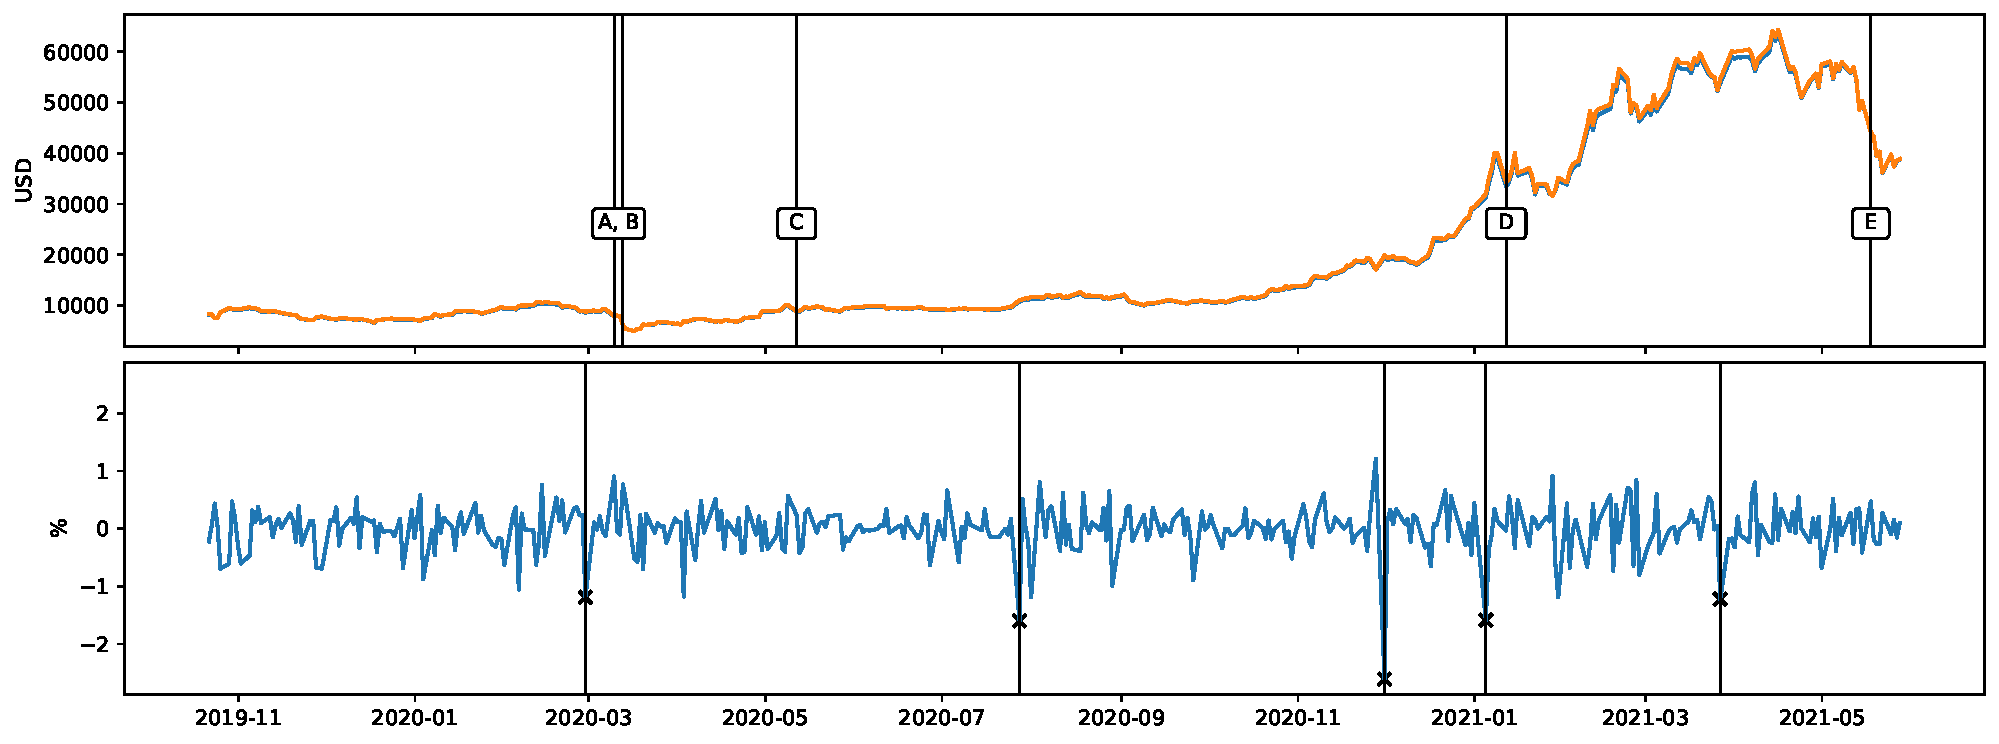
\includegraphics[width=\textwidth]{_pics/BTC_price.pdf}
  \caption{Out-of-sample BTC and BTCF price. The first panel presents the price of BTC in blue line and that of BTCF in orange line.
  The black vertical lines with capital letter labels indicate the five most negative daily return of BTC in the out-of-sample data.
  The second panel presents the difference between the percentage returns of BTC and BTCF.
  The black vertical lines indicate the five most negative returns.
  The crosses locate the level the returns.
 \href{https://github.com/QuantLet/Hedging-Cryptos-with-Bitcoin-Futures/blob/main/newToQuantlet/Pynotebooks/figures/Figure 3_4_5.ipynb}{\includegraphics[height=\baselineskip]{_pics/qletlogo_tr.png}} }
\label{fig:BTC_price}
\end{figure}

\begin{table}[!h]
    \centering
      \begin{tabularx}{.8\textwidth}{cccX}
        \toprule
        Label &   Date & \% Drop in Price &  Summary\\
        \midrule
        A &  2020-03-09 & 13.83 &  Coronavirus outbreak that affects
        the global markets; BTC as potential safe-haven was
        questioned.$^1$\\ 
        B &  2020-03-12 & 22.89 &  Continuation of the 2020-03-09
        drop.  \\ 
        C &  2020-05-11 & 12.11 &  Price correction (from \$10,000 to
        \$8,100) after BTC price surge because of the third supply
        halving.$^{2,3}$ \\ 
        D &  2021-01-11 & 14.41 &  Short term correction of BTC hits
        the \$40,000 mark.$^4$\\ 
        E &  2021-05-17 & 11.86 &  Tesla stops accepting BTC as
        payment currency due to environmental concerns related to the
        excessive energy use in processing transactions.$^5$\\ 
        \bottomrule
      \end{tabularx}
        \caption{Summary of events associated with the five most
          extreme daily price drops in out-of-sample BTC price data. 
        The capital letter labels in the first column correspond to
        the labels in the first panel of figure~\ref{fig:BTC_price}. 
        $^1$ is reported by the CNBC news \url{https://cnb.cx/3HZ2x7K}; $^2$ is from Forbes \url{https://bit.ly/3rdJPmP};
        $^3$ is from livemint.com \url{https://bit.ly/3FRi6Na};
        $^4$ is from CNBC \url{https://cnb.cx/3nU0ppO};
        $^5$ is from Reuters \url{https://reut.rs/3leCiAv}.
        }
        \label{tab:BTC_5min}
  \end{table}
\clearpage
\newpage

\begin{figure}[t]
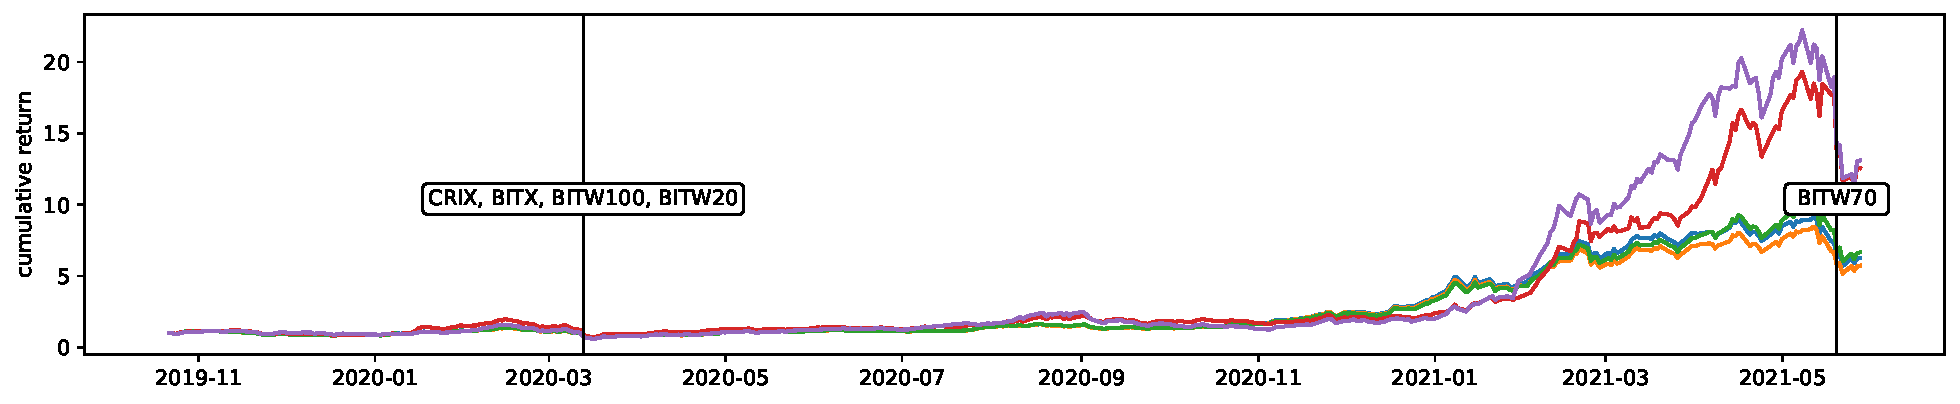
\includegraphics[width=\textwidth]{_pics/index_price.pdf}
  \caption{Out-of-sample cumulative returns of crypto indices. 
  The black vertical lines indicate the largest price drops of each
  index as indicated by the labels.
  The colouring is as follows:
  \textcolor{plt1}{Blue line} is CRIX;
  \textcolor{plt2}{Orange line} is BITX;
  \textcolor{plt3}{Green line} is BITW100;
  \textcolor{plt4}{Red line} is BITW20;
  \textcolor{plt5}{Purple line} is BITW70.
  \href{https://github.com/QuantLet/Hedging-Cryptos-with-Bitcoin-Futures/blob/main/newToQuantlet/Pynotebooks/figures/Figure 3_4_5.ipynb}{\includegraphics[height=\baselineskip]{_pics/qletlogo_tr.png}} }
  \label{fig:index_price}
\end{figure}

\begin{figure}[t]
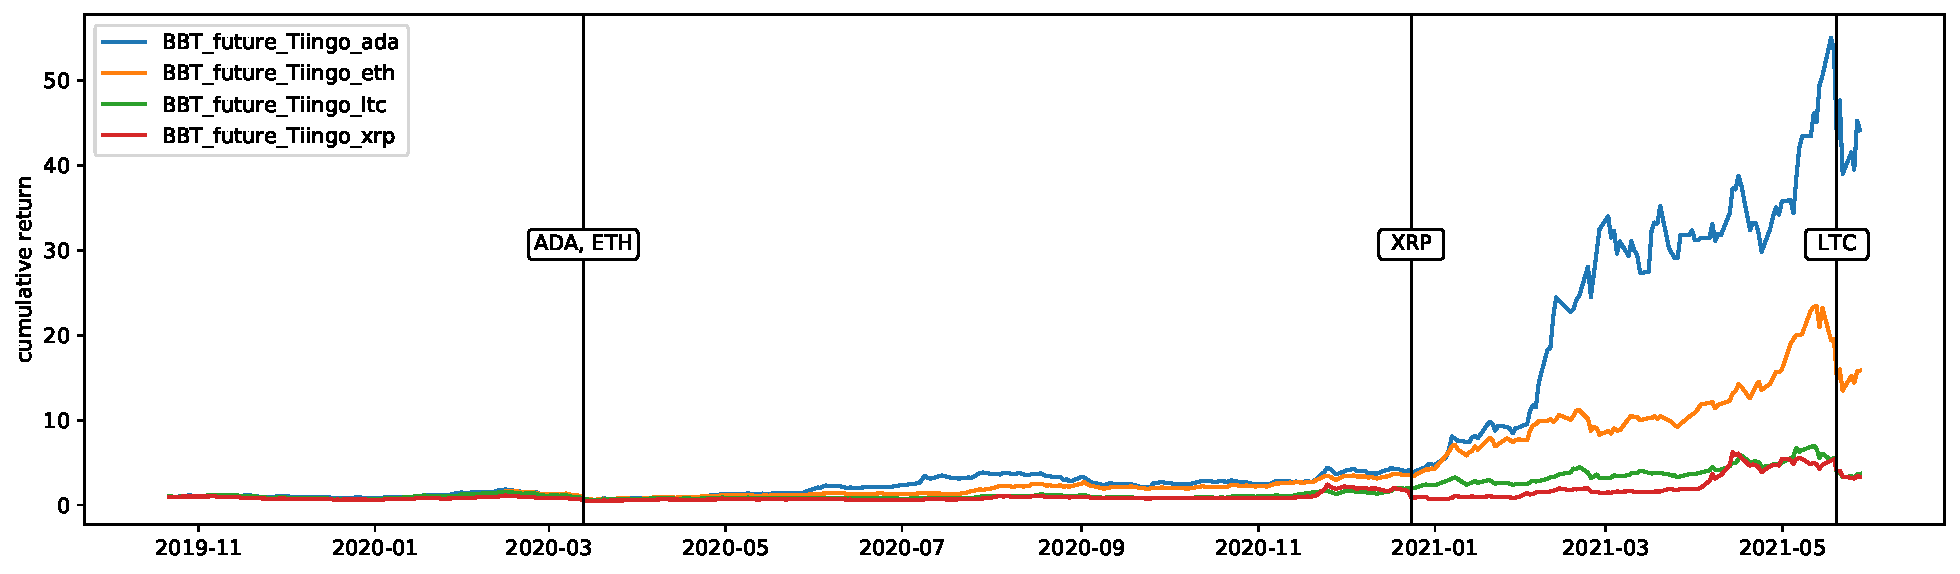
\includegraphics[width=\textwidth]{_pics/individualCoins_price.pdf}
  \caption{Out-of-sample cumulative returns of individual cyptos.
  The black vertical lines indicate the largest price drops each
  cryptos as indicated by the labels.
    \textcolor{plt1}{Blue line} is ADA;
  \textcolor{plt2}{Orange line} is ETH;
  \textcolor{plt3}{Green line} is LTC;
  \textcolor{plt4}{Red line} is XRP.
  \href{https://github.com/QuantLet/Hedging-Cryptos-with-Bitcoin-Futures/blob/main/newToQuantlet/Pynotebooks/figures/Figure 3_4_5.ipynb}{\includegraphics[height=\baselineskip]{_pics/qletlogo_tr.png}} }
  \label{fig:individualCoins_price}
\end{figure}

\begin{table}[t]
    \centering
      \begin{tabularx}{.8\textwidth}{cccX}
        \toprule
        Label &  Date & \% Drop in Price &  Summary\\
        \midrule
        CRIX    &2020-03-12 & 23.77 &
        \multirow[t]{6}{\hsize}{Coronavirus outbreak that affects the
          global markets including the crpyto market.}\\ 
        BITX    & & 23.68 &  \\
        BITW100 & & 23.87 &  \\
        BITW20  & & 26.66 &  \\
        ADA     & & 23.55 &  \\
        ETH     & & 27.40 &  \\
        BITW70  & 2021-05-19 & 27.64 & Spillover of the BTC shock on
        2021-05-17 (label A in Figure~\ref{fig:BTC_price} and
        Table~\ref{tab:BTC_5min})\\ 
        XRP     & 2020-12-23 & 41.00 & Top executives of Ripple Labs
        sued by the SEC of misleading investors$^1$. \\ 
        \bottomrule
      \end{tabularx}
        \caption{Summary of events that associated with largest price drops in out-of-sample data.
        The labels in the first column are the labels in Figure \ref{fig:index_price} and Figure \ref{fig:individualCoins_price}.
        CRIX, BITX, BITW100, BITW20, ADA and ETH have the same date
        the reason of the largest drop.$^1$ is reported by Bloomberg
        \url{https://bloom.bg/3cWdita}.} 
        \label{tab:All_min}
  \end{table}
\clearpage
\newpage
\subsection{An overview of the hedged portfolios without the copula
  selection step}
\label{subsec:HP1}
  \begin{figure}[t]
    \centering
    \begin{minipage}[t]{.475\textwidth}
        \centering
        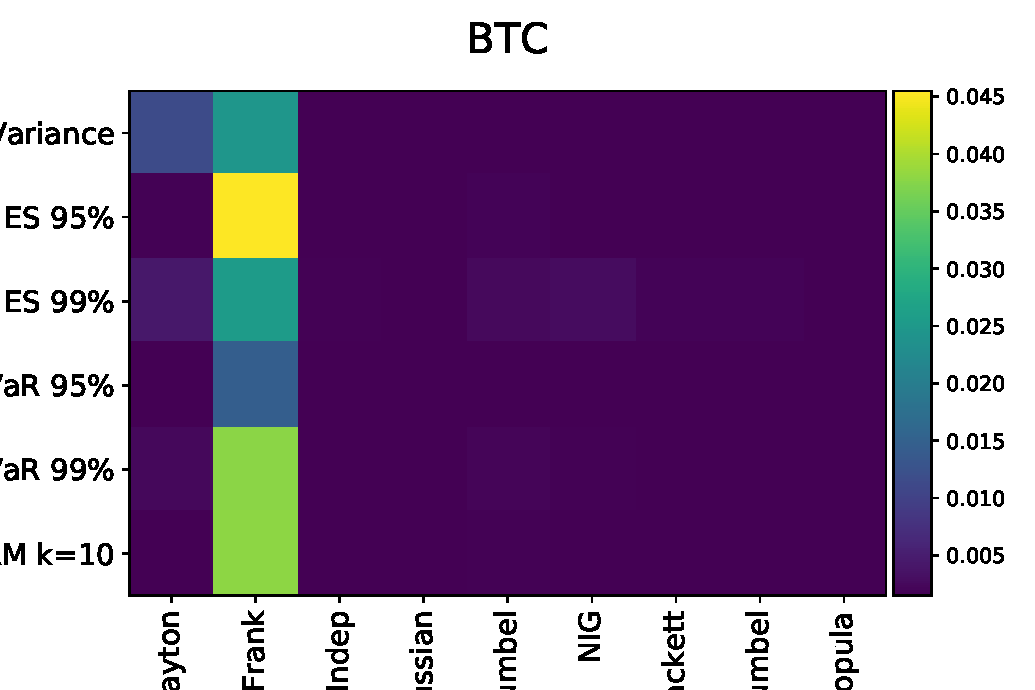
\includegraphics[width=\textwidth]{_pics/MSE_BTC.pdf}
      \caption{Out-of-sample mean square errors of BTC-BTCF portfolios constructed with different copula and risk minimization objectives.
        The Frank copula is inferior in the BTC-involved portfolios.
        \href{https://github.com/QuantLet/Hedging-Cryptos-with-Bitcoin-Futures/blob/main/newToQuantlet/Pynotebooks/figures/figure 6_7_8_9_10_11.ipynb}{\includegraphics[height=\baselineskip]{_pics/qletlogo_tr.png}} }
        \label{fig:MSE_BTC}
    \end{minipage}
    \hfill
    \begin{minipage}[t]{.475\textwidth}
        \centering
        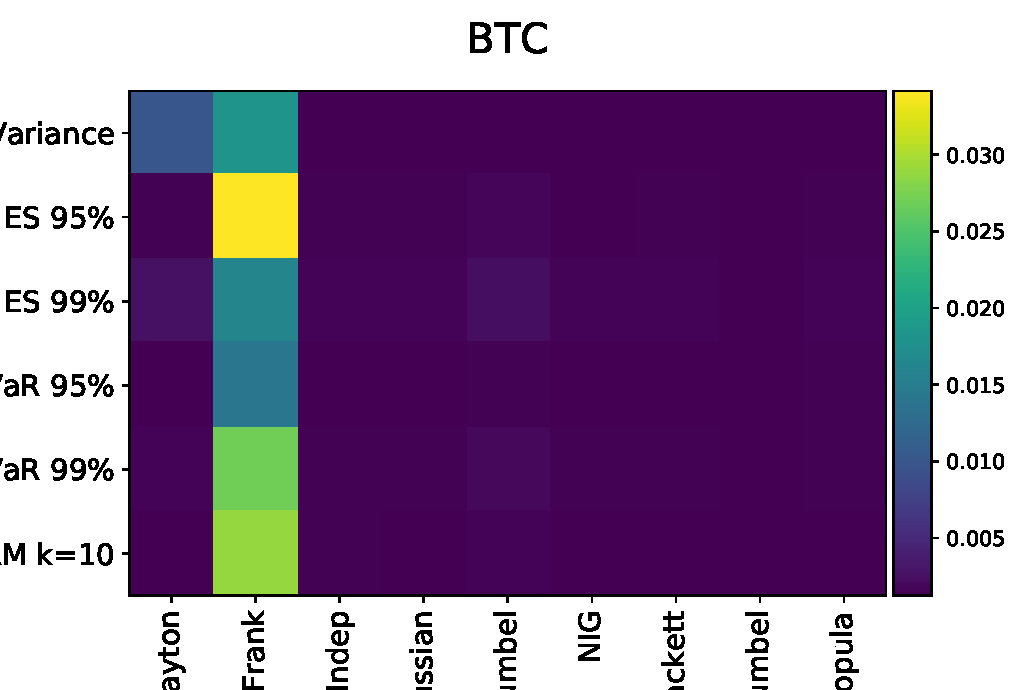
\includegraphics[width=\textwidth]{_pics/semiLowerVariance_BTC.pdf}
      \caption{Out-of-sample lower semivariance of BTC-BTCF portfolios constructed with different copula and risk minimization objectives.
      The Frank copula is obviously inferior.
      \href{https://github.com/QuantLet/Hedging-Cryptos-with-Bitcoin-Futures/blob/main/newToQuantlet/Pynotebooks/figures/figure 6_7_8_9_10_11.ipynb}{\includegraphics[height=\baselineskip]{_pics/qletlogo_tr.png}} }
      \label{fig:SLV_BTC}
    \end{minipage}
    \end{figure}  

First, we analyse the results of the hedged portfolios without the
copula selection step in order to get a better understanding of how a
copula affects the hedged portfolio with various risk minimization
objectives.
To do so, we inspect the hedge performance of copulas by
the mean square error and lower semi-variance.
The mean square error
is the distance between a perfect hedge and the hedged portfolio
returns $\operatorname{MSE}= \E(R^2)$.
The lower semi-variance is defined as
$\operatorname{LSV}=\E \left( (R-\E(R))^2 \1_{\{R\leq \E(R)\}} \right)$.
All results presented here are out-of-sample results obtained without
the copula selection step in order to compare the performances across
copulae.

Figures \ref{fig:MSE_BTC} to \ref{SLV_indices} visualise the out-of-sample MSEs and LSVs of all the portfolios in colorplots.
Figures \ref{fig:MSE_BTC} and \ref{fig:SLV_BTC} are the MSEs and LSVs of BTC-BTCF. 
By far, the Frank copula is the worst performing copula.
In Figures \ref{MSE_indices} and \ref{SLV_indices}, the phenomenon
of Frank copula being inferior to its counterparts can also be observed
from the results of the CRIX, BITX, BITW100, and BITW20-BTCF
portfolios.
Interestingly, the spot in those portfolios usually have a strong
dependence with the BTCF.
In contrast, the inferiority of the Frank copula is less prominent in
the BITW70, ADA, ETH, LTC and XRP-BTCF portfolios.

We suspect that the Frank copula is not a choice to model assets with
strong dependence.

From Figures \ref{MSE_cryptos} and
\ref{SLV_cryptos}, one can see that the Gumbel copula is not performing as well as
other copulas in the ETH, LTC, and XRP-BTCF portfolios.
The reason is the Gumbel copula has only upper tail dependence,
while the ETH, LTC, and XRP exhibit lower tail dependence with BTCF.

\newpage
\begin{landscape}
\begin{figure}[h]
  \begin{minipage}[t]{0.475\linewidth}
    \centering
    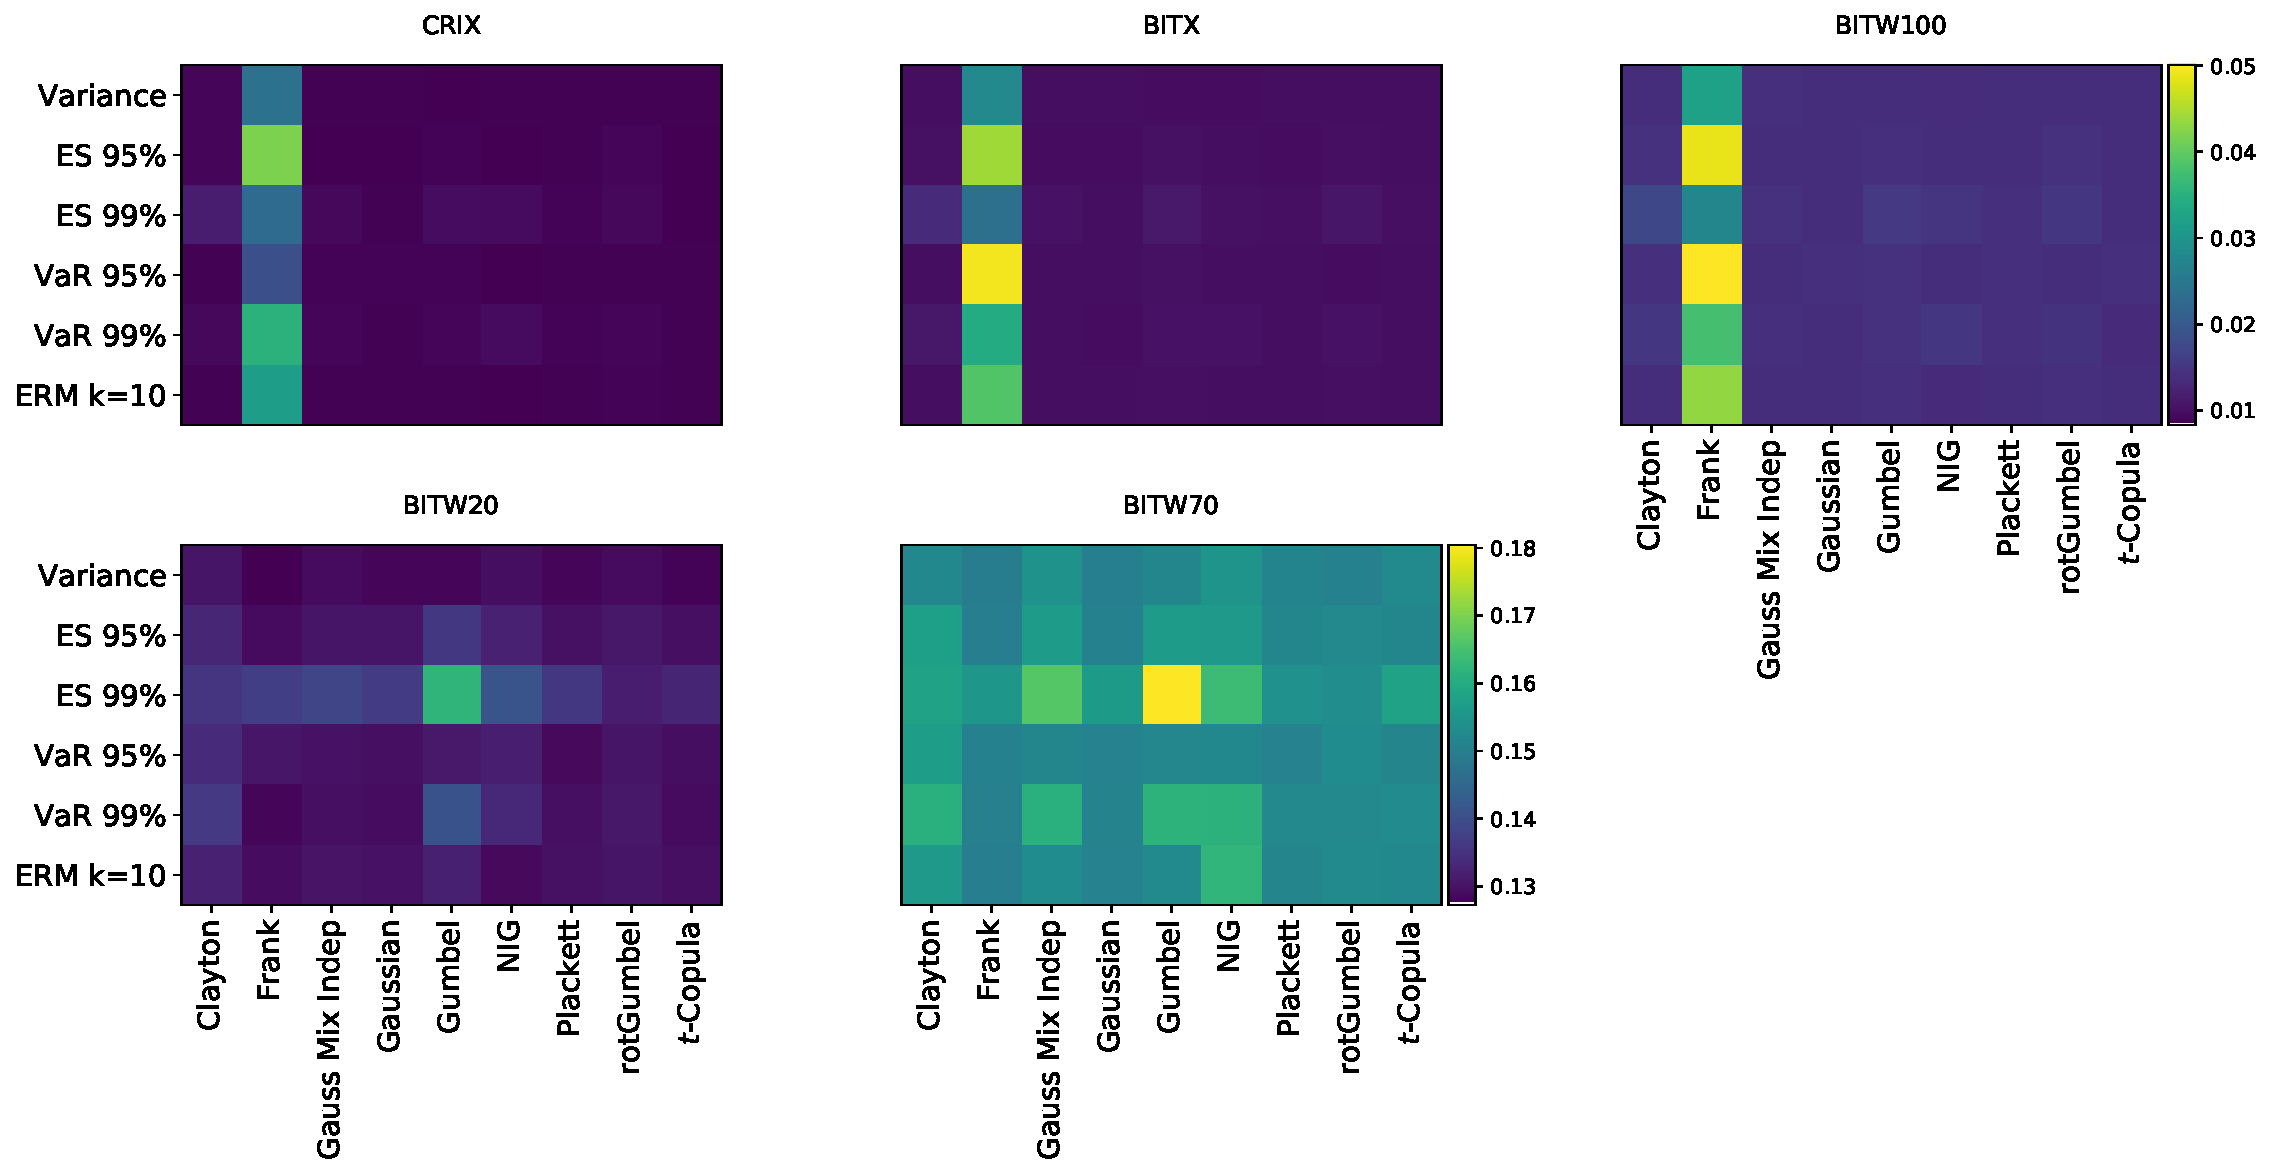
\includegraphics[height=.5\linewidth]{_pics/MSE_indices.pdf}
    \caption{Out-of-sample mean square errors of indices' hedge portfolios. Plots in a row share the same colour scale for comparison.
    \href{https://github.com/QuantLet/Hedging-Cryptos-with-Bitcoin-Futures/blob/main/newToQuantlet/Pynotebooks/figures/figure 6_7_8_9_10_11.ipynb}{\includegraphics[height=\baselineskip]{_pics/qletlogo_tr.png}}}
    \label{MSE_indices}
  \end{minipage}
  \hfill
  \begin{minipage}[t]{0.475\linewidth}
    \centering
    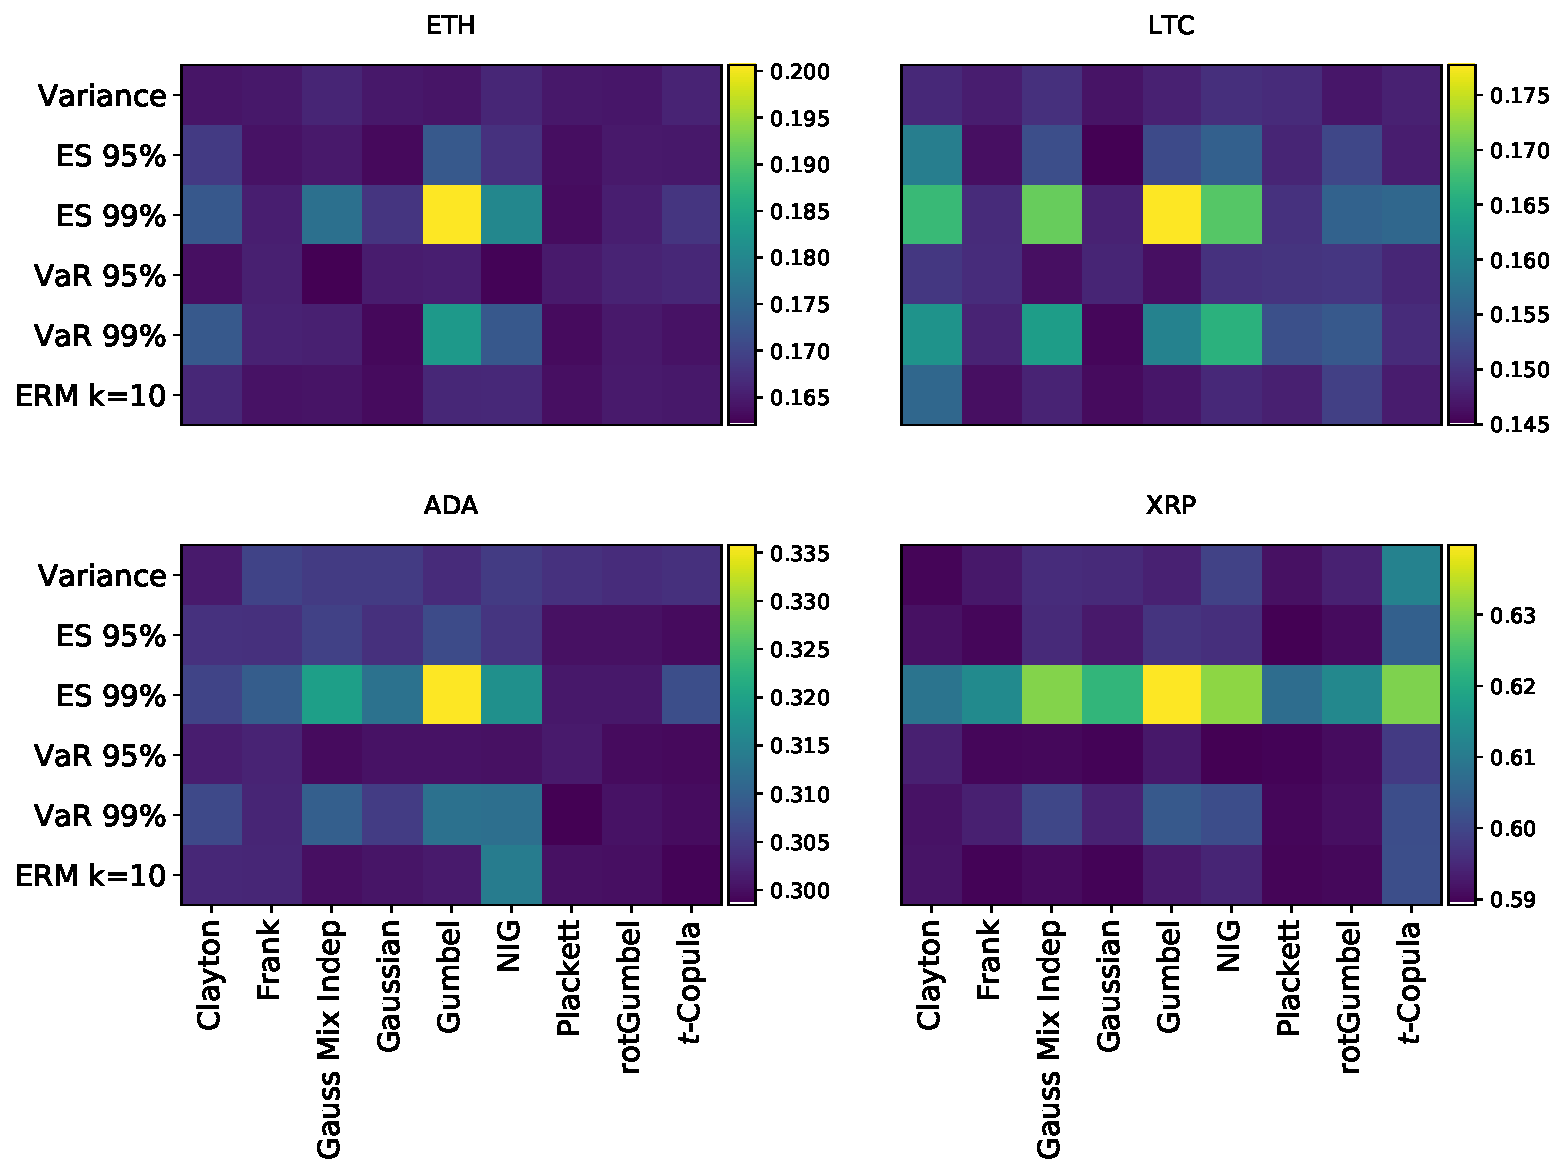
\includegraphics[height=.5\linewidth]{_pics/MSE_cryptos.pdf}
    \caption{Out-of-sample mean square errors of cryptos' hedge portfolios. Each plot has its own colour scale.
    \href{https://github.com/QuantLet/Hedging-Cryptos-with-Bitcoin-Futures/blob/main/newToQuantlet/Pynotebooks/figures/figure 6_7_8_9_10_11.ipynb}{\includegraphics[height=\baselineskip]{_pics/qletlogo_tr.png}}}\label{MSE_cryptos}
  \end{minipage}
  \begin{minipage}[b]{0.475\linewidth}
    \centering
    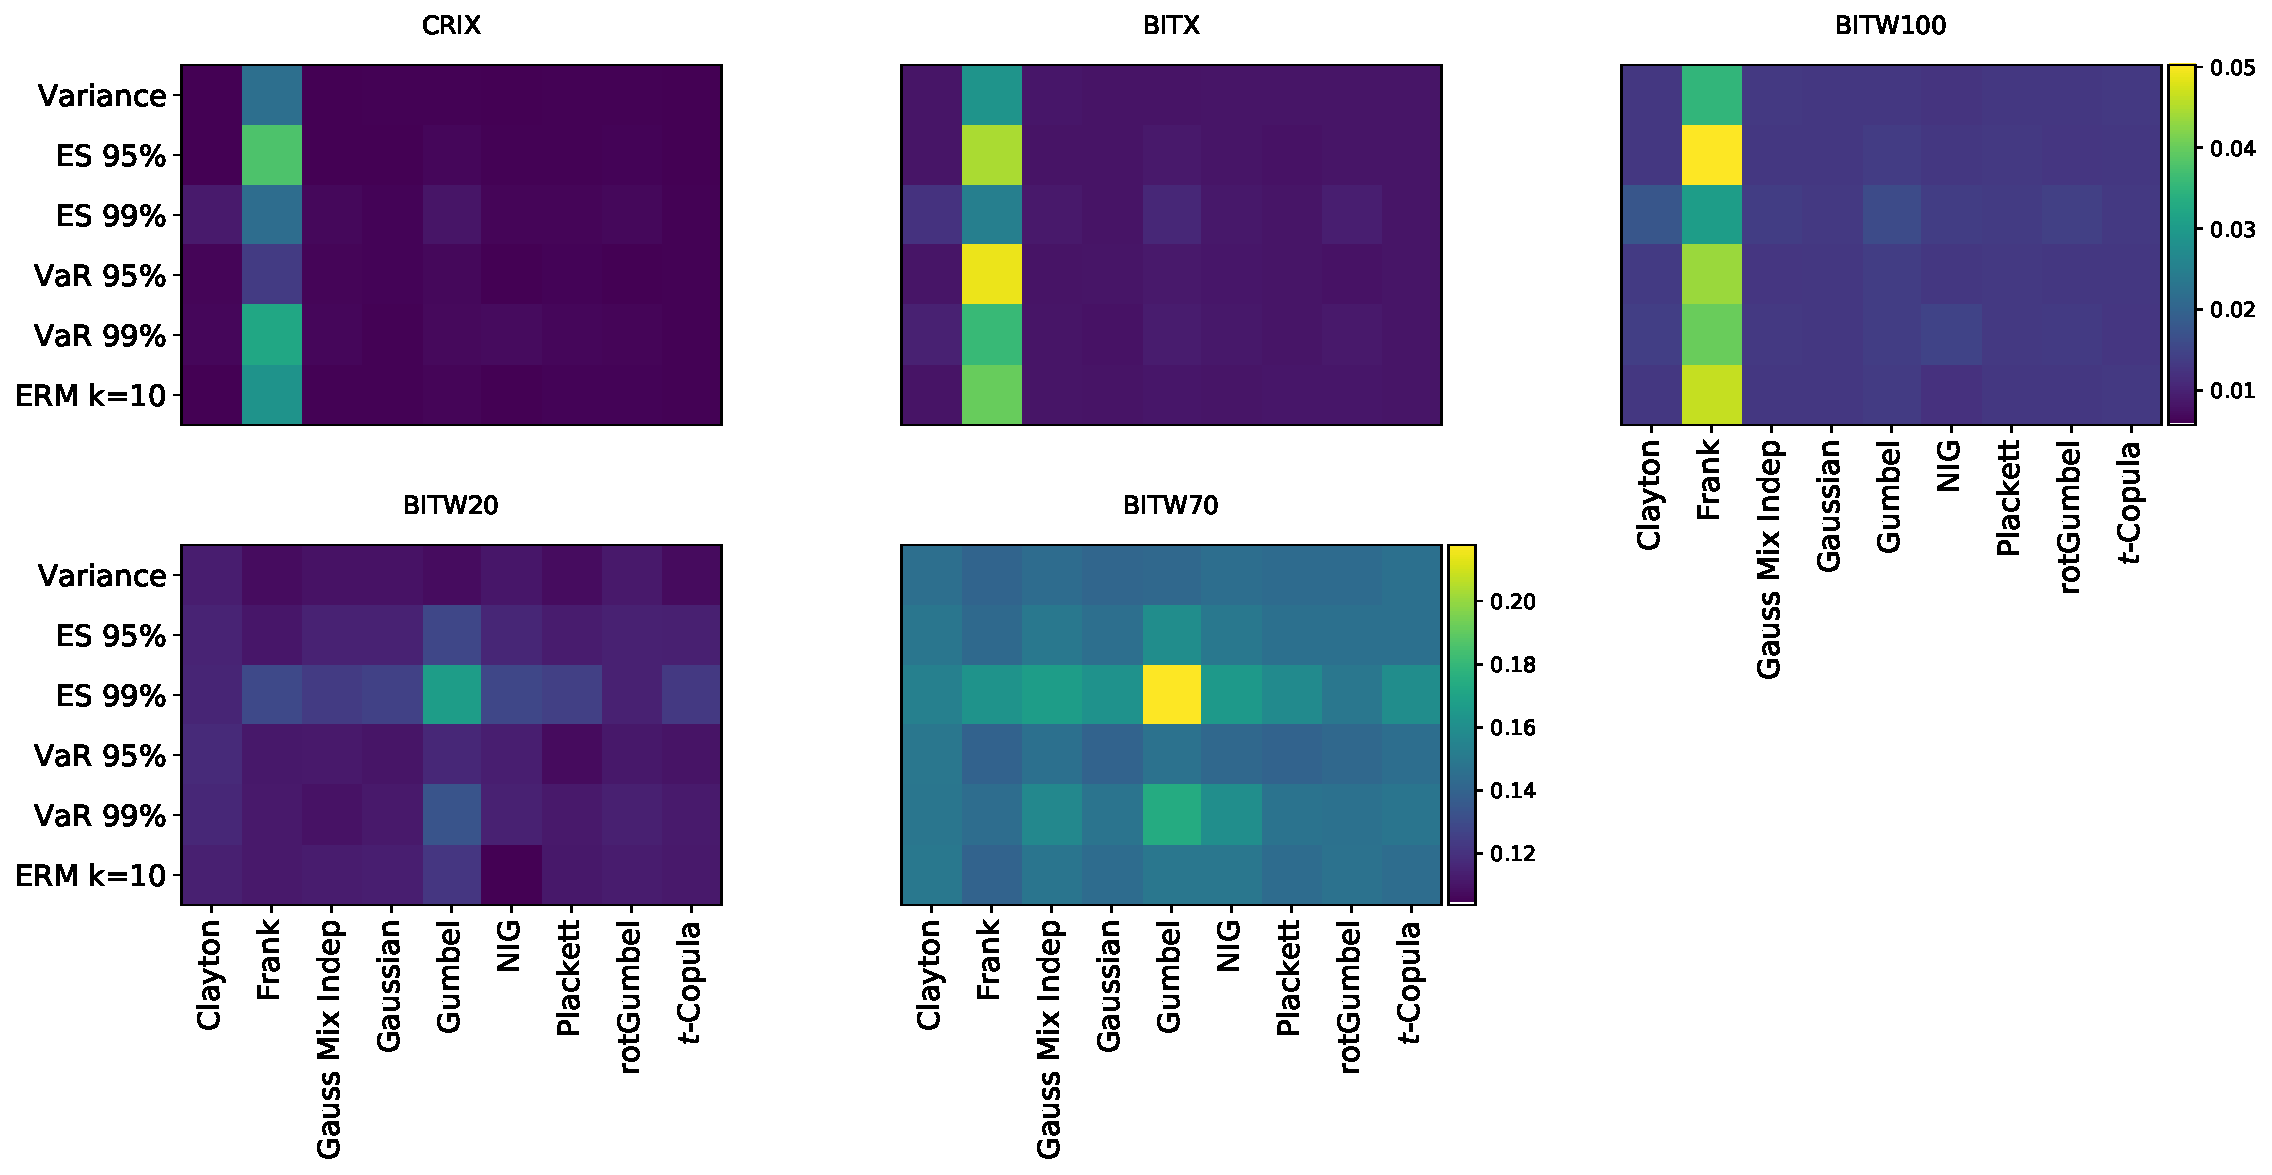
\includegraphics[height=.5\linewidth]{_pics/semiVariance_indices.pdf}
    \caption{Out-of-sample lower semi variance of indices' hedge portfolios. Plots in a row share the same colour scale for comparison.
    \href{https://github.com/QuantLet/Hedging-Cryptos-with-Bitcoin-Futures/blob/main/newToQuantlet/Pynotebooks/figures/figure 6_7_8_9_10_11.ipynb}{\includegraphics[height=\baselineskip]{_pics/qletlogo_tr.png}}}
    \label{SLV_cryptos}
  \end{minipage}
    \hfill
  \begin{minipage}[b]{0.475\linewidth}
    \centering
    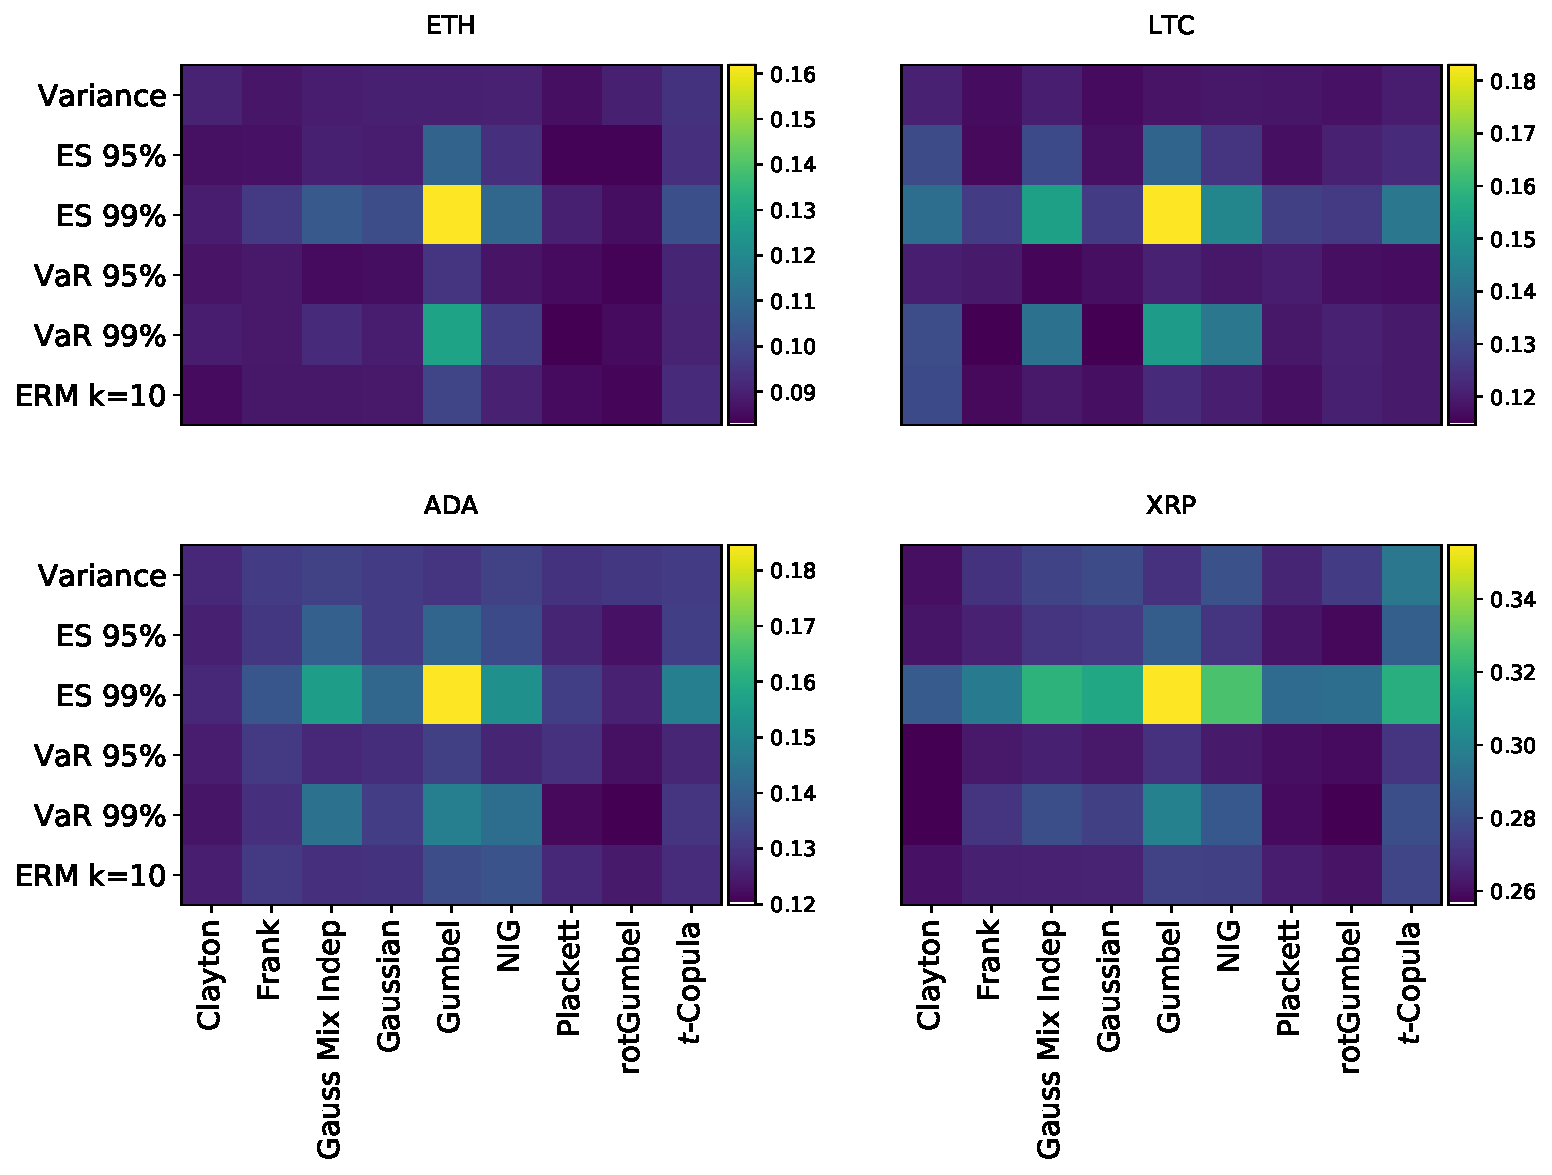
\includegraphics[height=.5\linewidth]{_pics/semiVariance_cryptos.pdf}
    \caption{Out-of-sample lower semi variance of cryptos' hedge portfolios. Each plot has its own colour scale.
    \href{https://github.com/QuantLet/Hedging-Cryptos-with-Bitcoin-Futures/blob/main/newToQuantlet/Pynotebooks/figures/figure 6_7_8_9_10_11.ipynb}{\includegraphics[height=\baselineskip]{_pics/qletlogo_tr.png}}}
    \label{SLV_indices}
  \end{minipage}
\end{figure}
\end{landscape}

\subsection{Copula Selection Results}\label{subsec:-copula-results}
\begin{table}[t]
  \centering
 \ra{1.1}
    {\begin{tabularx}{\textwidth}{lYYYYY} \toprule
         Copula/Asset & $t$ & Plackett & GMI & rotGumbel & NIG \\ \midrule
     \multicolumn{6}{l}{Individual Cryptos}                                                                                 \\
        \ \ \ BTC          & 73         & 4                 & 2                        & 1                  & 31                  \\
        \ \ \ ETH          & 3          & 6                 & 8                        & 94                 & 1                   \\
        \ \ \ ADA          & 0          & 0                 & 0                        & 0                  & 112                 \\
        \ \ \ LTC          & 13         & 0                 & 3                        & 32                 & 64                  \\
        \ \ \ XRP          & 0          & 31                & 3                        & 78                 & 0                   \\
   \multicolumn{6}{l}{Crypto Indices with BTC Constituent}                                                                  \\
        \ \ \ BITX         & 39         & 0                 & 14                       & 16                 & 12                  \\
        \ \ \ CRIX         & 47         & 0                 & 11                       & 3                  & 27                  \\
        \ \ \ BITW100      & 42         & 0                 & 8                        & 29                 & 2                   \\
    \multicolumn{6}{l}{Crypto Indices without BTC Constituent}                                                              \\
        \ \ \ BITW20       & 0          & 0                 & 0                        & 78                 & 3                   \\
        \ \ \ BITW70       & 0          & 0                 & 0                        & 80                 & 1                   \\
    \bottomrule
    \end{tabularx}
        \caption{Copula Selection Results. }









 \caption{Copula selection results (shortened).
        The values are the percentage of time of a copula chosen by
        the AIC procedure over the out-of-sample period. 
        The table shows only the frequently chosen copulas, which are
        $t$, Plackett, Gaussian Mix Independent (GMI), rotated Gumbel
        (rotGumbel) and Normal Inverse Gaussian factor copula (NIG). 
        }
    \label{tab:copulasection}
\end{table}
Next, we inspect the copula selection results by the AIC procedure
described in Section~\ref{subsec:copula-selection}. 
Although the copula selection is only an intermediate step to obtain
the optimal hedge ratios,
the result of this step can help us better understand the dependence
feature between BTCF and the assets we study in this work.
This provides valuable information for modeling the assets in the future.
The decisions of the AIC procedure are summarised in Table
\ref{tab:copulasection}. Overall, the $t$-copula, rotated Gumbel
(rotGumbel), and the NIG factor copula are the most frequently chosen
copulae by the AIC procedure.

The $t$-copula is predominantly chosen by the AIC procedure to model the dependence between 
the BTC and BTC-involving-indices, CRIX, BITX, BITW100, and the BTC
future.
BTC and BTC-involving-indices exhibit strong (upper and lower) tail
dependence with BTCF, a strong tendency for one asset to be extreme when the other is extreme and
vice versa. 
See \cite{McNeil2015} for further details about tail dependence.
In fact, the $t$ copula has been recommended in various empirical
studies to model financial data, such as~\cite{zeevi2002beyond} and~
\cite{breymann2003dependence}.
Those studies suggest that the $t$-copula is a better model compared
to the Gaussian copula as financial data typically exhibit heavy tails
and tail dependence. 

On the other hand, the symmetric $t$-copula appears to be 
a poor choice to model the remaining hedging pairs. 
\cite{demarta2005t} describes the symmetry feature of the $t$-copula ``strong'':
if $(U_1, ..., U_d)$ is a vector distributed in $t$-copula,
then $(U_1, ..., U_d) \overset{\mathcal{L}}= (1-U_1, ...,1-U_d)$.

Here, the AIC criterion predominantly selects copulas that allow for asymmetry between the spot
and the BTCF.
This reflects that overall asymetric dependence between a non-BTC-related spot asset and
the BTCF.
In fact, we observe from the crypto market that asset prices tend to crash simultaneously whereas positive development
tends to be idiosyncratic.   

Among the three popular copulae, rotGumbel copula shows its ability to
model the dependence between ETH and BTCF. rotGumbel also performs
well when modelling dependence between XRP, BITW20, BITW70, and the
BTCF. In particular, the whole time series of the two indices, BITW20
and BITW70, are best fitted solely with the rotated Gumbel
copula.

In fact, Clayton's AIC in many of the training sets is the second
lowest, just slightly higher than that of rotated Gumbel. This is because the
Clayton copula has the same ability to model the lower quantile
dependence. However, Clayton's radial like feature does not match the
behaviour of the financial data. 

It is worth to mention that although the NIG factor copula is
penalised heavily due to its three parameters setup, it is frequently
chosen to be the best copula to model the dependence between
individual cryptos and the BTC future. An extreme case occurs for ADA,
where only the NIG factor is chosen in our dataset. 
Another dependence structure best described by the NIG factor
copula is the pair of LTC-BTCF, with 64 out of 112 training sets best
fitted by the NIG factor copula. Indices like BITX and CRIX are
sometimes best fitted with the NIG factor copula as well, accounting
for modelling 12 and 27 training sets, respectively. 
The popularity of the NIG factor copula reflects the ability of the
copula to model complex dependence structure, involving heavier tails
than the Gaussian as well as asymmetric distributions.

The Frank copula turn out to generally be a poor choice to model financial
data (as also reported by \cite{barbi2014copula}).
The Plackett copula is characterised by its dependence parameter being
equal to the cross-product ratio, see
(\ref{eq:PlackettCrossProduct}). However, this property
does not capture the dependence structure of cryptos and BTCF.

\subsection{Hedged portfolios with the copula selection step}\label{subsec:HP2}

\afterpage{
  \begin{landscape}
  \begin{table}[!] \centering
\resizebox{.8\paperheight}{!}{%
\begin{tabular}{l*{10}{r}}
\toprule
{} &   BTC & ETH & ADA & LTC & XRP & BITX & CRIX & BITW100 & BITW20 & BITW70\\
\midrule
  \multicolumn{10}{l}{Spots assets only}   \\
\ \ \ Mean \%  &      0.3915 &      0.6819 &      0.9467 &      0.3227 &      0.2987 &      0.4308 &      0.4602 &      0.4683 &      0.6249 &      0.6353 \\
\ \ \ Std \%   &      4.4023 &      6.0103 &       6.699 &      6.4781 &      7.9843 &      4.5676 &       4.542 &      4.6174 &      5.5021 &      5.8155 \\
\ \ \ MD \%    &    -25.9965 &    -32.0144 &    -26.8528 &    -37.5913 &    -52.7652 &     -27.022 &    -27.1385 &    -27.2694 &    -31.0092 &    -32.3453 \\
\ \ \ MD date &  2020-03-12 &  2020-03-12 &  2020-03-12 &  2021-05-19 &  2020-12-23 &  2020-03-12 &  2020-03-12 &  2020-03-12 &  2020-03-12 &  2021-05-19 \\
  \multicolumn{10}{l}{Variance minimizing portfolios}   \\
\ \ \ Mean \%  &      0.0215 &      0.2823 &      0.5617 &     -0.0871 &     -0.0123 &      0.0561 &      0.0812 &      0.0855 &      0.2429 &      0.2706 \\
\ \ \ Std \%   &      0.3221 &      3.8741 &      5.2722 &      3.9052 &      7.1537 &      0.9954 &      0.9183 &      1.1986 &      3.5846 &      3.8838 \\
\ \ \ MD \%    &     -1.4393 &    -17.7421 &    -13.8687 &    -28.3029 &    -52.5236 &     -7.7567 &     -7.1025 &    -11.3866 &     -21.468 &    -23.9984 \\
\ \ \ MD date &  2020-11-30 &  2021-05-19 &  2021-01-08 &  2021-05-19 &  2020-12-23 &  2021-05-19 &  2021-05-19 &  2021-05-19 &  2021-05-19 &  2021-05-19 \\
  \multicolumn{10}{l}{VaR 95\% minimizing portfolios}   \\
\ \ \ Mean \%  &      0.0253 &      0.3084 &      0.5726 &     -0.0742 &      0.0208 &      0.0562 &      0.0863 &      0.0846 &      0.2728 &      0.2847 \\
\ \ \ Std \%   &      0.3294 &      3.8944 &      5.2204 &      3.9145 &       7.152 &       0.993 &      0.9151 &       1.198 &       3.594 &      3.9133 \\
\ \ \ MD \%    &     -1.5347 &     -19.175 &    -14.6974 &    -28.3672 &    -52.5667 &     -7.5639 &     -6.9744 &    -11.2582 &    -22.0733 &    -24.6513 \\
\ \ \ MD date &  2020-11-30 &  2021-05-19 &  2021-05-19 &  2021-05-19 &  2020-12-23 &  2021-05-19 &  2021-05-19 &  2021-05-19 &  2021-05-19 &  2021-05-19 \\
  \multicolumn{10}{l}{VaR 99\% minimizing portfolios}   \\
\ \ \ Mean \%  &      0.0176 &      0.2977 &      0.5562 &     -0.0852 &      0.0352 &      0.0593 &      0.0738 &      0.0823 &      0.2499 &      0.2788 \\
\ \ \ Std \%   &       0.327 &      3.9132 &      5.3466 &      4.1503 &      7.1658 &      1.0178 &      0.9695 &      1.2338 &       3.621 &      3.9257 \\
\ \ \ MD \%    &     -1.5689 &    -18.6061 &    -15.4795 &    -29.0915 &    -52.5727 &     -8.0299 &     -7.0185 &    -11.8752 &    -21.6634 &    -24.5294 \\
\ \ \ MD date &  2020-11-30 &  2021-05-19 &  2021-05-19 &  2021-05-19 &  2020-12-23 &  2021-05-19 &  2021-05-19 &  2021-05-19 &  2021-05-19 &  2021-05-19 \\
  \multicolumn{10}{l}{ES 95\% minimizing portfolios}   \\
\ \ \ Mean \%  &      0.0204 &      0.3082 &      0.5525 &     -0.0808 &      0.0176 &      0.0591 &      0.0777 &      0.0848 &      0.2608 &      0.2785 \\
\ \ \ Std \%   &      0.3234 &       3.889 &      5.2673 &      3.9829 &      7.1533 &      1.0065 &      0.9207 &      1.2125 &      3.6115 &      3.9157 \\
\ \ \ MD \%    &     -1.5629 &    -18.7819 &    -14.9647 &    -28.4608 &    -52.5698 &     -7.6211 &     -6.9894 &    -11.1357 &     -21.543 &    -24.3474 \\
\ \ \ MD date &  2020-11-30 &  2021-05-19 &  2021-05-19 &  2021-05-19 &  2020-12-23 &  2021-05-19 &  2021-05-19 &  2021-05-19 &  2021-05-19 &  2021-05-19 \\
  \multicolumn{10}{l}{ES 99\% minimizing portfolios}   \\
\ \ \ Mean \%  &      0.0148 &       0.308 &      0.5016 &     -0.1029 &       -0.02 &      0.0598 &      0.0835 &      0.0781 &      0.2538 &       0.266 \\
\ \ \ Std \%   &      0.3476 &      3.8954 &       5.404 &      4.1581 &      7.2887 &      1.0312 &      0.9461 &       1.264 &      3.6323 &       3.932 \\
\ \ \ MD \%    &     -1.6225 &    -18.7625 &    -15.4481 &    -29.1727 &      -52.57 &     -7.7424 &     -7.0203 &    -11.9263 &    -21.9866 &    -24.4764 \\
\ \ \ MD date &  2020-11-30 &  2021-05-19 &  2021-05-19 &  2021-05-19 &  2020-12-23 &  2021-05-19 &  2021-05-19 &  2021-05-19 &  2021-05-19 &  2021-05-19 \\
  \multicolumn{10}{l}{ERM $k=10$ minimizing portfolios}   \\
\ \ \ Mean \%  &      0.0223 &      0.3117 &      0.5722 &     -0.0512 &      0.0155 &       0.059 &       0.084 &      0.0853 &      0.2564 &      0.2818 \\
\ \ \ Std \%   &      0.3221 &      3.8679 &       5.359 &      3.8812 &      7.1579 &      1.0078 &      0.9087 &      1.2032 &      3.6009 &      3.9074 \\
\ \ \ MD \%    &     -1.5242 &    -18.8729 &    -14.3885 &    -28.0879 &    -52.5689 &     -7.8581 &      -7.053 &    -11.1846 &     -21.592 &     -24.525 \\
\ \ \ MD date &  2020-11-30 &  2021-05-19 &  2021-01-08 &  2021-05-19 &  2020-12-23 &  2021-05-19 &  2021-05-19 &  2021-05-19 &  2021-05-19 &  2021-05-19 \\
\bottomrule
\end{tabular}}
\end{table}
\end{landscape}
}

We now turn to the hedge performance. 
Table~\ref{tab:bigTable}
presents the first two moments, maximum drawdown (MD) and the date of
MD of the hedge portfolios. An interesting observation is the similarity of
the statistics when minimising with respect to different risk measures.
Detailed statistics are in Tables~\ref{tab:var_rh} to \ref{tab:ERM_rh} in Appendix
\ref{appendix:summary_stats}. 
 
Unsurprisingly, the BTC-involved spots, i.e., BTC, CRIX, BITX, and
BITW100, are well hedged by the BTCF regardless of risk minimization
objective. 
The BTC-not-involved spots, on the contrary, are less promising. Those
hedge portfolios' returns are nearly as volatile as the
assets themselves, see for example ADA and XRP. 
We further discuss the effectiveness of hedge in the next
section. %\ref{sec: HE results}. 

\subsection{Hedging Effectiveness Results}\label{sec: HE results}
In this section, we analyse the out-of-sample hedging effectiveness
(HE) of BTCF as a hedge instrument. 
HE is defined as $$\text{HE} = 1-\frac{\rho_h}{\rho_s},$$
i.e., it measures the percentage reduction of risk of the hedge
portfolio $\rho_h $ relative to the risk of the spot position $\rho_s$.
A higher HE indicates a greater risk reduction and thus the hedge is
more effective.  
The HE above is a generalisation of how \citet{ederington1979hedging}
evaluates hedge performance, which focusses on variance as the risk
measure. 
Aside from variance, we include the risk measures which act as
loss function while searching for the optimal hedge ratios: ES 95\%
and 99\%, VaR 95\% and 99\% and ERM.

\begin{figure}[t]
  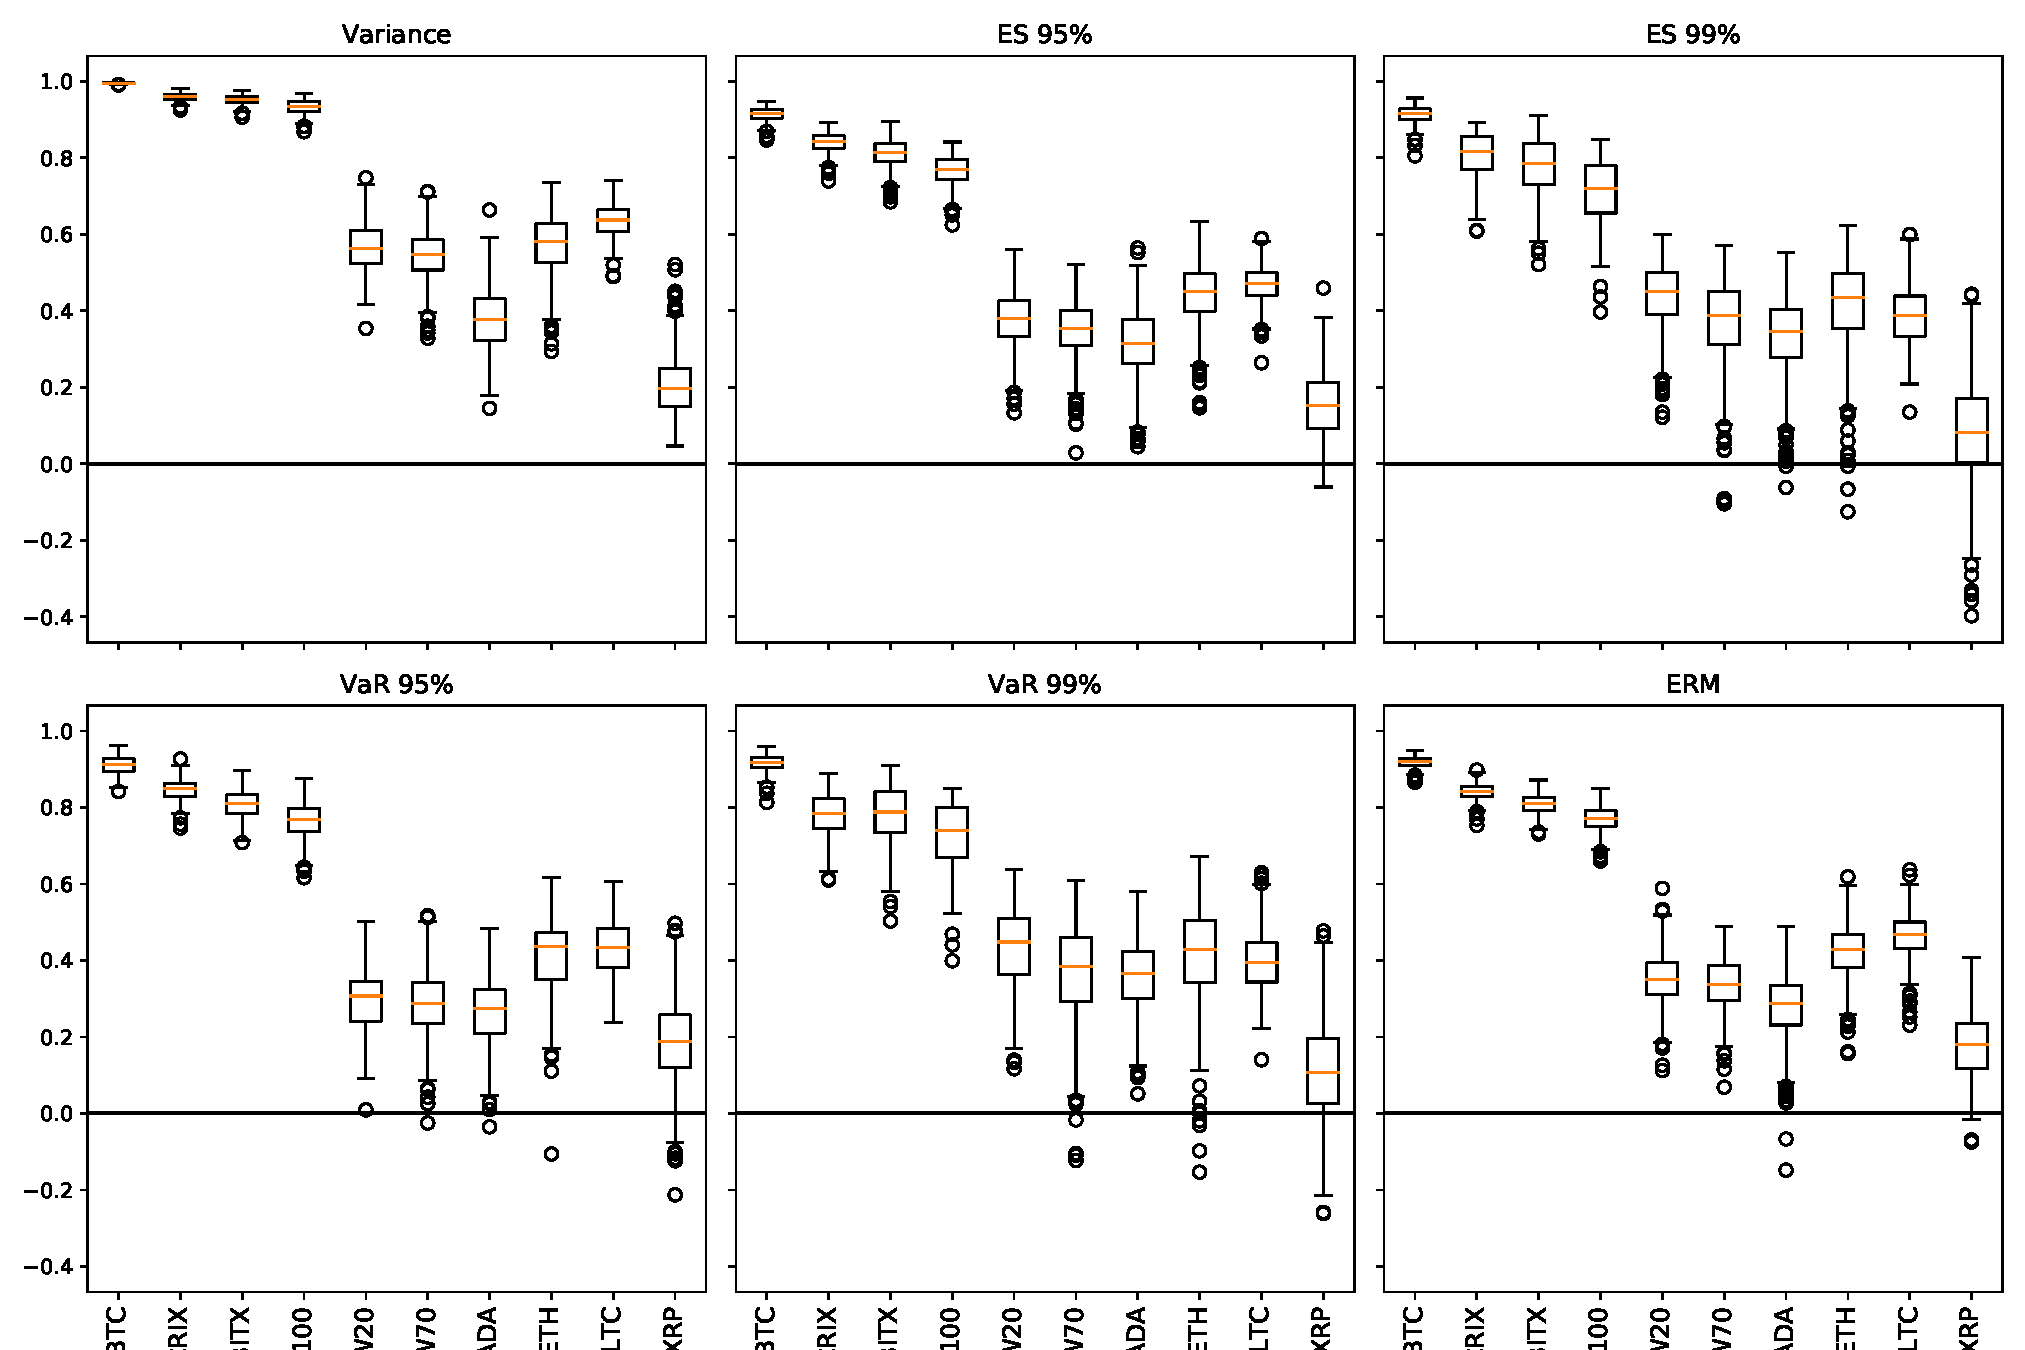
\includegraphics[width=\textwidth]{_pics/HE_boxplot.pdf}
    \caption{Hedging effectiveness (HE) of portfolios with different risk minimization objectives evaluated by the corresponding risk minimization objectives.
              The boxplots indicate the the median, upper quartile, lower quartile, minimium and maximum of the bootstrapped HE.
              The HE of BTC-involved spots are significantly higher than that of BTC-not-involved spots.
    \href{https://github.com/QuantLet/Hedging-Cryptos-with-Bitcoin-Futures/blob/main/newToQuantlet/Pynotebooks/figures/figure 12.ipynb}{\includegraphics[height=\baselineskip]{_pics/qletlogo_tr.png}}
    }
    \label{fig:HEboxplot}
  \end{figure}

As described in Section \ref{sec:empirical-procedure}, the backtesting procedure gives
an out-of-sample hedged portfolio return time series for every spot-copula-risk measure combination. 
The time series represent the profit and lost if hedgers recalibrate copulae and adjust the hedge ratio every 5 days.  
In order to obtain a robust HE result (instead of a point estimate), we apply the bootstrapping method.
Bootstrapping refers to sampling from the empirical distribution of a
given data sample (e.g.\ a time series of fiancial returns). The
principal idea underlying bootstrapping is to provide statistical
information about estimators that cannot be derived from just one
realisation of the data. The method was introduced by
\cite{Efron1979}; see also \citep{efron1994introduction, davison1997bootstrap}. 

A specific type of bootstrapping method designed for timeseries, namely the stationary block bootstrap \cite{Politis1994}, is applied in our analysis.
The stationary bootstrapping procedure is as follows. 
Assume a time series $\{X_t\}_{t \in [1,N]}$ that is
a stationary weakly time dependent time series,
 we first draw a block of samples $\{X_i, ..., X_{i+j-1}\}$, where the index $i$ is a
random variable uniformly distributed over 
$[1,2,...,N]$ and $j$ is geometric distributed random variable with
parameter $p$ independent of $i$. 
For any index $k$ which is greater than $N$, the sample $X_k$ is
defined to be $X_{k(\mathrm{mod} N)}$. 
Then, we repeat the procedure until the number of samples are drawn in total across the blocks equal or exceed a predefined sample length $S$. 
One bootstrapped time series sample is then the concantenation of the blocks truncated to length of $S$.
The resulting bootstrapped time series is known as pseudo time series. 

We choose $p=1/5$, implying the average block length is 5 such that it aligns with the recalibration frequency. 
The length of each pseudo time series sample $S = 300$ is chosen to be aligned with the length of each training set.  
The length of each pseudo time series sample allows ES and VaR to be calculated in a reasonable length.
We draw in total $n=500$ pseudo time series,
for each of them we compute various HE measures to obtain a collection of HE samples. 

Figure \ref{fig:HEboxplot} reports the bootstrapped HE samples.
As expected, the BTC involving spots, the BTC, CRIX, BITX and BITW100, are well hedged
by the BTCF. 
The HEs of the other cryptos and indices are
substantially lower than to the BTC-related instruments, but 
exhibit a consistent performances across different risk measures. 
As it turns out, some HE bootstrapping samples are even negative,
which means the "hedge" portfolio actually increases the risk. 
This shows BTC futures is not suitable for cross-asset hedges (cross hedge).
In fact, in the previous study by \citet{corbet2018bitcoin}, 
researchers yield negative hedging effectiveness even when hedging against BTC exposure.
% \citet{} show that derivatives in BitMEX



\section{Conclusion and Outlook}\label{sec:conclusion-and-outlook}
We study the effectiveness of hedging cryptos and crypto indices with
Bitcoin futures.
To accommodate different risk appetites and scenarios, a variety of
commonly used risk measures are considered to determine the optimal
hedge ratio. The risk measures comprise variance, value-at-risk at
the confidence levels 95\% and 99\%, expected shortfall 95\% and 99\%,
and the exponential risk measure with parameter $k=10$.

At the time of writing, the crypto market is a vibrant and
fast-developing market, causing cryptos to have complex and
time-changing dependence structures with the Bitcoin futures.
As a consequence, the dependence between the cryptos and the futures
contract plays an important role in hedging as it determines the
distribution of the portfolio returns. We therefore consider various
copulae, a flexible statistical tool that separates modelling of the
marginals and the dependence structure of multivariate random
vectors. To address the potential time-changing dependence, we
periodically re-calibrate the copula models and determine the
best-fitting copula via AIC. 

An extensive out-of-sample backtest suggests that the CME Bitcoin futures
are consistently capable of hedging BTC and BTC-involved indices,
i.e., BITX, CRIX, and BITW100, under different risk minimisation
objectives 
and copula models. The mean-square errors (MSEs) and lower
semi-variances (LSVs) of the resulting portfolios are
indistinguishable at a low level except for the Frank copula. 
For BTC-related spot asset, the AIC procedure consistently
pick the $t$-copula because it  
captures the tail dependence feature of the data. 
Compared to the unhedged cases, the
portfolios' out-of-sample maximum drawdowns are significantly reduced. 

Contrarily, we observe diverse results of the capability of BTC
futures to hedge other cryptos and crypto indices that exclude Bitcoin. 
In general, ES 95\% and VaR 95\% perform better than their 99\%
in terms of mean square error (MSE) and lower semi variance (LSV).
In particular, minimising ES 99\% leads to relatively
high MSEs and LSVs regardless of the copula in use. The ES 99\% and
VaR 99\% even result in out-of-sample maximum drawdowns that are
higher than that of the 95\% counterparts in some portfolios, 
for example in the ETH- and LTC-BTCF portfolios.
Therefore, we conclude that overly emphasising tail risks by choosing
extreme tail risk measures does not lead to a promising hedge in a
cross-hedging setting. 

As an intermediate step in determining the optimal hedge ratio, we report also the results from the AIC procedure.
The procedure mainly favours the rotated Gumbel and the NIG
factor copula while modelling non-BTC relate cryptos and indices. This
reflects the systematic nature of 
downward movements in the crypto market. Interestingly, the best-fitting
copula does not necessary lead to the best performing portfolio in
terms of MSE or LSV. This is the case, for example, for ADA. 
We suspect that this discrepancy between the optimal copula selection and
MSE-LSV results can be attributed to the static linear nature of the
hedge, as the sole hedge instrument is a futures contract; the
hedge is not sophisticated enough to react to the more involved
dependence structure.

With further analysis, the conclusion drawn from this study can also be applied to crypto market related policy making.
Our results connect to the discussion of whether authority should allow crypto futures hedge as basis to lower the minimum capital requirements inflicted by crypto exposure.
While the debates carry on at the time of writing
\footnote{See the Basel Committee on Banking Supervision proposals and consultative documents about prudential treatment of banks' crypto-asset exposures from \url{https://www.bis.org/bcbs/publ/d533.htm}.}
, our results align and can be seen as an extension of the existing researches made by stakeholders,
for example, research done by CME \footnote{See the CME and KPMG's reports on \url{https://www.cmegroup.com/education/files/basics-of-hedge-effectiveness.pdf}.},
and International Swaps and Derivatives Association's report \footnote{See the ISDA report "Crypto-asset Risks and Hedging Analysis" on \url{https://www.isda.org/a/pMWgE/Crypto-asset-Risks-and-Hedging-Analysis.pdf}.}.
Nonetheless, further studies are required to rule out or understand the risks other than market risk, e.g. operation risk and counterparty risk. 
On the other hand, our results provide partial evidences in supporting separate regulatory treatments of cryptos with a matured regulated derivatives market and those without. 
Our results show a clear distinction between the hedging effectiveness of BTC futures to BTC related assets and BTC unrelated assets. 
Hedgers are empowered by the BTC futures to manage their BTC and BTC-related exposure, but not the other crypto exposures.
Further studies are required to generalise the hedging effectiveness of other crypto-futures pairs. 

\clearpage
%
\bibliography{finance} %
\appendix
\section{Density of linear combination of random variables}
\label{sec:appendix}
\begin{proposition}
   Let $\bm{X} = (X_1, ..., X_d)^\top$ be real-valued random variables with corresponding
   copula density $\bm{c}_{X_1, ..., X_d}$, and continuous marginals $F_{X_1}, ..., F_{X_d}$.
   Then, the
   pdf of the linear combination of marginals $Z = n_1 \cdot X_1 +
   ... +  n_d \cdot X_d $ is
   \begin{align}
   f_Z(z) &= \left| n_1^{-1} \right| \int_{[0,1]^{d-1}} \bm{c}_{X_1,...,X_d}
      \left(F_{X_1} (S(z)), u_2, ..., u_d \right) \cdot
      f_{X_1} (S(z)) \dd u_2 ... \dd u_d, \label{density}
   \end{align}
   with
   \begin{align*}
      S(z) &= \frac{1}{n_1}\cdot z - \frac{n_2}{n_1} \cdot F^{(-1)}_{X_2}(u_2) - ... -  \frac{n_d}{n_1} \cdot F^{(-1)}_{X_d}(u_d).
      \end{align*}
   \end{proposition}

\begin{proof}
  Let
    \[\mathbf A=\displaystyle \begin{bmatrix}
      n_1    & n_2  & \cdots &    & n_d     \\
      0      & 1    & \cdots  &    & 0       \\
      0      & 0    & 1 &  \cdots & 0       \\
      \vdots &      & & \ddots & \vdots \\
      0      & \cdots &       & 1  \\
    \end{bmatrix}.\]
    Then,
    \begin{equation*}
      \begin{bmatrix}
        Z \\ X_2 \\ \vdots \\ X_d
      \end{bmatrix}
      = \bm{A}
      \begin{bmatrix}
         X_1 \\ X_2 \\ \vdots \\ X_d
      \end{bmatrix}.
    \end{equation*}

   By transformation of the variables~\citep[Section 4.3]{hardle2019applied},
   \begin{align*}
      \bm{f}_{Z,X_2,...,X_d}(z, x_2, ...,x_d) &= \bm{f}_{X_1,...,X_d}\left( \bm{A}^{-1}
      \begin{bmatrix}
         z \\ x_2 \\ \vdots \\ x_d
      \end{bmatrix}
      \right)  \cdot |\det \bm{A}^{-1}| \\
      &= \left| n_1^{-1} \right| \bm{f}_{X_1,...,X_d}\left(S(z), x_2,...,x_d\right).
      \end{align*} \medskip

   Let $u_i = F_{X_i}(x_i)$. By chain rule we have
   \begin{align*}
       \bm{f}_{X_1,...,X_d}(x_1,...,x_d) &= \frac{\partial^d F_{X_1,...,X_d}(x_1, ..., x_d)}{\partial x_1 ... \partial x_d}\\
                                         &= \bm{c}_{X_1,...,X_d}(u_1, ..., u_d) \cdot \prod_{i=1}^d f_{X_i}(x_i).
   \end{align*}

    Therefore,
   \begin{align*}
      \bm{f}_{Z,X_2,...,X_d}&(z, x_2, ...,x_d) = \\
       \left| n_1^{-1} \right| &\cdot
      \bm{c}_{X_1,...,X_d}\left(F_{X_1}( S(z)), u_2, ...,  u_d\right)  \cdot
      f_{X_1} \{ S(z) \} \cdot
      \prod_{i=2}^d f_{X_i}(x_i).
      \end{align*}

   The claim (\ref{density}) is obtained by integrating out $x_2, ... x_d$ by substituting $\dd x_i = \frac{1}{f_{X_i}(x_i)} \dd u_i$.
   \end{proof}

\section{Summary Statistics}\label{appendix:summary_stats}

{\small %
  \begin{table}[th] \centering %\resizebox{\textwidth}{!}
    {%
\begin{tabular}{lrrrrrrrr} \toprule
         {} &    Mean \% &     Std \% &      Skew &       Kurt &         MD \% &     MD date & $\rho$ & $\tau$ \\
\midrule
     \multicolumn{9}{l}{Hedging Instrument} \\
\ \ \ BTCF    &  0.3906 &  4.6312 & -0.5060 &   4.4204 & -26.9920 &  2020-03-12 &  1.0000 &  1.0000 \\
     \multicolumn{9}{l}{Individual Cryptos}                                                                                 \\
\ \ \ BTC     &  0.3915 &  4.4023 & -0.5857 &   4.6565 & -25.9965 &  2020-03-12 &  0.9975 &  0.9507 \\
\ \ \ ETH     &  0.6819 &  6.0103 & -0.2557 &   5.2646 & -32.0144 &  2020-03-12 &  0.7712 &  0.5988 \\
\ \ \ ADA     &  0.9467 &  6.6990 &  0.1661 &   2.3086 & -26.8528 &  2020-03-12 &  0.6296 &  0.4825 \\
\ \ \ LTC     &  0.3227 &  6.4781 & -0.9935 &   5.3011 & -37.5913 &  2021-05-19 &  0.8080 &  0.6113 \\
\ \ \ XRP     &  0.2987 &  7.9843 &  0.5542 &  12.4882 & -52.7652 &  2020-12-23 &  0.4510 &  0.4939 \\
   \multicolumn{9}{l}{Crypto Indices with BTC Constituent}                                                                  \\
\ \ \ BITX    &  0.4308 &  4.5676 & -0.8842 &   4.7222 & -27.0220 &  2020-03-12 &  0.9769 &  0.8738 \\
\ \ \ CRIX    &  0.4602 &  4.5420 & -0.7952 &   4.7549 & -27.1385 &  2020-03-12 &  0.9799 &  0.8769 \\
\ \ \ BITW100 &  0.4683 &  4.6174 & -0.9864 &   4.9381 & -27.2694 &  2020-03-12 &  0.9674 &  0.8537 \\
    \multicolumn{9}{l}{Crypto Indices without BTC Constituent}                                                              \\
\ \ \ BITW20  &  0.6249 &  5.5021 & -1.1518 &   5.2203 & -31.0092 &  2020-03-12 &  0.7674 &  0.5883 \\
\ \ \ BITW70  &  0.6353 &  5.8155 & -1.1171 &   5.1926 & -32.3453 &  2021-05-19 &  0.7525 &  0.5459 \\
\bottomrule
\end{tabular}}
\caption{Summary statistics of assets' daily returns during the out-of-sample period, from 2019-10-21 to 2021-05-27.
        The first four columns are the first four moments of assets' daily returns.
        The fifth and sixth columns are the maximum drawdown (MD) and the date of the MD.
        The last two columns are Pearson's $\rho$s and Kendall's $\tau$s between the assets and BTCF. }
\label{tab:SSA}

\end{table}
}

\clearpage
\newpage
% \section{Summary Statistics of Hedged Portfolios}\label{sec:SSHP}
{\small %
  \begin{table}[h] \centering %\resizebox{\textwidth}{!}
    {%
\begin{tabular}{lrrrrrrr} \toprule
         {} &    Mean \% &     Std \% &      Skew &       Kurt &         MD \% &     MD date & Variance \\
\midrule
     \multicolumn{7}{l}{Individual Cryptos}                                                                                 \\
\ \ \ BTC     &  0.0215 &  0.3221 & -1.0119 &   3.1929 &  -1.4393 &  2020-11-30 &    0.0000 \\
\ \ \ ETH     &  0.2823 &  3.8741 &  0.9469 &   7.1064 & -17.7421 &  2021-05-19 &    0.0015 \\
\ \ \ ADA     &  0.5617 &  5.2722 &  1.3634 &   4.4818 & -13.8687 &  2021-01-08 &    0.0028 \\
\ \ \ LTC     & -0.0871 &  3.9052 & -0.3617 &   7.6239 & -28.3029 &  2021-05-19 &    0.0018 \\
\ \ \ XRP     & -0.0123 &  7.1537 &  1.1451 &  20.0236 & -52.5236 &  2020-12-23 &    0.0043 \\
   \multicolumn{7}{l}{Crypto Indices with BTC Constituent}                                                                  \\
\ \ \ BITX    &  0.0561 &  0.9954 & -0.4204 &  13.2487 &  -7.7567 &  2021-05-19 &    0.0001 \\
\ \ \ CRIX    &  0.0812 &  0.9183 & -0.0027 &  14.3136 &  -7.1025 &  2021-05-19 &    0.0001 \\
\ \ \ BITW100 &  0.0855 &  1.1986 & -1.7440 &  22.2644 & -11.3866 &  2021-05-19 &    0.0001 \\
    \multicolumn{7}{l}{Crypto Indices without BTC Constituent}                                                              \\
\ \ \ BITW20  &  0.2429 &  3.5846 & -0.3063 &   4.1622 & -21.4680 &  2021-05-19 &    0.0013 \\
\ \ \ BITW70  &  0.2706 &  3.8838 & -0.6490 &   4.6312 & -23.9984 &  2021-05-19 &    0.0015 \\
\bottomrule
\end{tabular}}
\caption{Summary statistics of out-of-sample daily returns of hedged portfolios that minimize variance.}
\label{tab:var_rh}

\end{table}\begin{table}[!] \centering %\resizebox{\textwidth}{!}
  {%
\begin{tabular}{lrrrrrrr} \toprule
         {} &    Mean \% &     Std \% &      Skew &       Kurt &         MD \% &     MD date & VaR 5\% \\
\midrule
     \multicolumn{7}{l}{Individual Cryptos}                                                                                 \\
\ \ \ BTC     &  0.0253 &  0.3294 & -0.9725 &   3.4373 &  -1.5347 &  2020-11-30 &  0.0063 \\
\ \ \ ETH     &  0.3084 &  3.8944 &  1.0243 &   7.4297 & -19.1750 &  2021-05-19 &  0.0514 \\
\ \ \ ADA     &  0.5726 &  5.2204 &  1.2981 &   4.2544 & -14.6974 &  2021-05-19 &  0.0769 \\
\ \ \ LTC     & -0.0742 &  3.9145 & -0.3836 &   7.5384 & -28.3672 &  2021-05-19 &  0.0622 \\
\ \ \ XRP     &  0.0208 &  7.1520 &  1.1269 &  19.8930 & -52.5667 &  2020-12-23 &  0.0683 \\
   \multicolumn{7}{l}{Crypto Indices with BTC Constituent}                                                                  \\
\ \ \ BITX    &  0.0562 &  0.9930 & -0.3117 &  12.4780 &  -7.5639 &  2021-05-19 &  0.0128 \\
\ \ \ CRIX    &  0.0863 &  0.9151 &  0.0718 &  13.7915 &  -6.9744 &  2021-05-19 &  0.0092 \\
\ \ \ BITW100 &  0.0846 &  1.1980 & -1.6592 &  21.3725 & -11.2582 &  2021-05-19 &  0.0164 \\
    \multicolumn{7}{l}{Crypto Indices without BTC Constituent}                                                              \\
\ \ \ BITW20  &  0.2728 &  3.5940 & -0.3721 &   4.4896 & -22.0733 &  2021-05-19 &  0.0546 \\
\ \ \ BITW70  &  0.2847 &  3.9133 & -0.6580 &   4.7874 & -24.6513 &  2021-05-19 &  0.0626 \\
\bottomrule
\end{tabular}}
\caption{Summary statistics of out-of-sample daily returns of hedged portfolios that minimize VaR 5\%.}
\label{tab:VaR5_rh}

\end{table}\begin{table}[!] \centering %\resizebox{\textwidth}{!}
  {%
\begin{tabular}{lrrrrrrr} \toprule
         {} &    Mean \% &     Std \% &      Skew &       Kurt &         MD \% &     MD date & VaR 1\% \\
\midrule
     \multicolumn{7}{l}{Individual Cryptos}                                                                                 \\
\ \ \ BTC     &  0.0176 &  0.3270 & -1.0405 &   3.3742 &  -1.5689 &  2020-11-30 &  0.0134 \\
\ \ \ ETH     &  0.2977 &  3.9132 &  0.9547 &   7.2414 & -18.6061 &  2021-05-19 &  0.1026 \\
\ \ \ ADA     &  0.5562 &  5.3466 &  1.1362 &   3.9334 & -15.4795 &  2021-05-19 &  0.1106 \\
\ \ \ LTC     & -0.0852 &  4.1503 & -0.7234 &   7.3208 & -29.0915 &  2021-05-19 &  0.1030 \\
\ \ \ XRP     &  0.0352 &  7.1658 &  1.1582 &  19.8506 & -52.5727 &  2020-12-23 &  0.1387 \\
   \multicolumn{7}{l}{Crypto Indices with BTC Constituent}                                                                  \\
\ \ \ BITX    &  0.0593 &  1.0178 & -0.5331 &  13.3100 &  -8.0299 &  2021-05-19 &  0.0247 \\
\ \ \ CRIX    &  0.0738 &  0.9695 & -0.4729 &  13.6500 &  -7.0185 &  2021-05-19 &  0.0245 \\
\ \ \ BITW100 &  0.0823 &  1.2338 & -1.9365 &  23.1938 & -11.8752 &  2021-05-19 &  0.0347 \\
    \multicolumn{7}{l}{Crypto Indices without BTC Constituent}                                                              \\
\ \ \ BITW20  &  0.2499 &  3.6210 & -0.3866 &   4.3396 & -21.6634 &  2021-05-19 &  0.0988 \\
\ \ \ BITW70  &  0.2788 &  3.9257 & -0.7635 &   5.1288 & -24.5294 &  2021-05-19 &  0.1147 \\
\bottomrule
\end{tabular}}
\caption{Summary statistics of out-of-sample daily returns of hedged portfolios that minimize VaR 1\%.}
\label{tab:VaR1_rh}

\end{table}\begin{table}[!] \centering %\resizebox{\textwidth}{!}
  {%
\begin{tabular}{lrrrrrrr} \toprule
         {} &    Mean \% &     Std \% &      Skew &       Kurt &         MD \% &     MD date & ES 5\% \\
\midrule
     \multicolumn{7}{l}{Individual Cryptos}                                                                                 \\
\ \ \ BTC     &  0.0204 &  0.3234 & -1.0150 &   3.4423 &  -1.5629 &  2020-11-30 &  0.0101 \\
\ \ \ ETH     &  0.3082 &  3.8890 &  1.0119 &   7.4077 & -18.7819 &  2021-05-19 &  0.0782 \\
\ \ \ ADA     &  0.5525 &  5.2673 &  1.2557 &   4.2423 & -14.9647 &  2021-05-19 &  0.0984 \\
\ \ \ LTC     & -0.0808 &  3.9829 & -0.4957 &   7.2302 & -28.4608 &  2021-05-19 &  0.0962 \\
\ \ \ XRP     &  0.0176 &  7.1533 &  1.1411 &  19.9176 & -52.5698 &  2020-12-23 &  0.1354 \\
   \multicolumn{7}{l}{Crypto Indices with BTC Constituent}                                                                  \\
\ \ \ BITX    &  0.0591 &  1.0065 & -0.3453 &  12.1335 &  -7.6211 &  2021-05-19 &  0.0215 \\
\ \ \ CRIX    &  0.0777 &  0.9207 &  0.0164 &  13.5608 &  -6.9894 &  2021-05-19 &  0.0173 \\
\ \ \ BITW100 &  0.0848 &  1.2125 & -1.6397 &  19.7472 & -11.1357 &  2021-05-19 &  0.0274 \\
    \multicolumn{7}{l}{Crypto Indices without BTC Constituent}                                                              \\
\ \ \ BITW20  &  0.2608 &  3.6115 & -0.3555 &   4.2016 & -21.5430 &  2021-05-19 &  0.0804 \\
\ \ \ BITW70  &  0.2785 &  3.9157 & -0.6949 &   4.8047 & -24.3474 &  2021-05-19 &  0.0908 \\
\bottomrule
\end{tabular}}
\caption{Summary statistics of out-of-sample daily returns of hedged portfolios that minimize ES 5\%.}
\label{tab:ES5_rh}

\end{table}\begin{table}[!] \centering %\resizebox{\textwidth}{!}
  {%
\begin{tabular}{lrrrrrrr} \toprule
         {} &    Mean \% &     Std \% &      Skew &       Kurt &         MD \% &     MD date & ES 1\% \\
\midrule
     \multicolumn{7}{l}{Individual Cryptos}                                                                                 \\
\ \ \ BTC     &  0.0148 &  0.3476 & -0.8354 &   3.3054 &  -1.6225 &  2020-11-30 &  0.0234 \\
\ \ \ ETH     &  0.3080 &  3.8954 &  0.9840 &   7.4947 & -18.7625 &  2021-05-19 &  0.1299 \\
\ \ \ ADA     &  0.5016 &  5.4040 &  1.1008 &   3.9607 & -15.4481 &  2021-05-19 &  0.1463 \\
\ \ \ LTC     & -0.1029 &  4.1581 & -0.7757 &   7.4375 & -29.1727 &  2021-05-19 &  0.1647 \\
\ \ \ XRP     & -0.0200 &  7.2887 &  1.1121 &  18.8732 & -52.5700 &  2020-12-23 &  0.2516 \\
   \multicolumn{7}{l}{Crypto Indices with BTC Constituent}                                                                  \\
\ \ \ BITX    &  0.0598 &  1.0312 & -0.4410 &  11.5863 &  -7.7424 &  2021-05-19 &  0.0411 \\
\ \ \ CRIX    &  0.0835 &  0.9461 & -0.0361 &  12.4047 &  -7.0203 &  2021-05-19 &  0.0350 \\
\ \ \ BITW100 &  0.0781 &  1.2640 & -1.9645 &  21.8836 & -11.9263 &  2021-05-19 &  0.0593 \\
    \multicolumn{7}{l}{Crypto Indices without BTC Constituent}                                                              \\
\ \ \ BITW20  &  0.2538 &  3.6323 & -0.4086 &   4.4462 & -21.9866 &  2021-05-19 &  0.1282 \\
\ \ \ BITW70  &  0.2660 &  3.9320 & -0.7598 &   5.0050 & -24.4764 &  2021-05-19 &  0.1535 \\
\bottomrule
\end{tabular}
}
\caption{Summary statistics of out-of-sample daily returns of hedged portfolios that minimize ES 1\%.}
\label{tab:ES1_rh}

\end{table}\begin{table}[!] \centering %\resizebox{\textwidth}{!}
  {%
\begin{tabular}{lrrrrrrr} \toprule
         {} &    Mean \% &     Std \% &      Skew &       Kurt &         MD \% &     MD date & ERM k=10 \\
\midrule
     \multicolumn{7}{l}{Individual Cryptos}                                                                                 \\
\ \ \ BTC     &  0.0223 &  0.3221 & -1.0008 &   3.4153 &  -1.5242 &  2020-11-30 &    0.0057 \\
\ \ \ ETH     &  0.3117 &  3.8679 &  1.0345 &   7.5751 & -18.8729 &  2021-05-19 &    0.0491 \\
\ \ \ ADA     &  0.5722 &  5.3590 &  1.4203 &   4.6970 & -14.3885 &  2021-01-08 &    0.0700 \\
\ \ \ LTC     & -0.0512 &  3.8812 & -0.2929 &   7.7022 & -28.0879 &  2021-05-19 &    0.0616 \\
\ \ \ XRP     &  0.0155 &  7.1579 &  1.1244 &  19.8583 & -52.5689 &  2020-12-23 &    0.0787 \\
   \multicolumn{7}{l}{Crypto Indices with BTC Constituent}                                                                  \\
\ \ \ BITX    &  0.0590 &  1.0078 & -0.4427 &  13.0839 &  -7.8581 &  2021-05-19 &    0.0127 \\
\ \ \ CRIX    &  0.0840 &  0.9087 &  0.0488 &  14.5501 &  -7.0530 &  2021-05-19 &    0.0100 \\
\ \ \ BITW100 &  0.0853 &  1.2032 & -1.6522 &  20.5562 & -11.1846 &  2021-05-19 &    0.0153 \\
    \multicolumn{7}{l}{Crypto Indices without BTC Constituent}                                                              \\
\ \ \ BITW20  &  0.2564 &  3.6009 & -0.3446 &   4.2152 & -21.5920 &  2021-05-19 &    0.0503 \\
\ \ \ BITW70  &  0.2818 &  3.9074 & -0.6952 &   4.8745 & -24.5250 &  2021-05-19 &    0.0557 \\
\bottomrule
\end{tabular}}
\caption{Summary statistics of out-of-sample daily returns of hedged portfolios that minimize ERM $k=10$.}
\label{tab:ERM_rh}

\end{table}
}

\clearpage
\section{Supplementary Material: Intraday Hedging}\label{sec:intraday}
Here we extend the hedging effectiveness analysis to intraday data again through backtesting.
BTC and ETH are chosen as spot to be hedged against by BTCF. 
The backtesting procedure in this section is the same to that of the main body, except the followings:
\begin{enumerate}
  \item recalibration and rebalancing frequencies are increased to every 4 hours,
  \item lengths of training data and test data are changed to 336 (equivalent to 14 days) and 4 respectively, and
  \item the stationary bootstrapping parameters are changed to $p=1/4, T=336, S=1000$ to adapt to the new rebalancing frequency. 
\end{enumerate}

The increased recalibration and rebalancing frequencies require hourly data that CME does not provide, 
causing us to backtest with data from less regulated crypto exchanges.

We collect price data from Deribit from 2020-06-01 00:00 UTC to 2020-08-01 00:00 UTC. 
All price data are hourly data.
The Deribit contract BTC-25SEP20 represents BTCF;
the Deribit BTC and ETH index represent the spot of BTC and ETH, respectively.
We take the hourly closing mid-price of the BTC-25SEP20 as the futures price and the last value of the BTC and ETH index in every hourly bucket as the spot prices.
Since the date range of the data is fully covered by the lifetime of BTC-25SEP20, this study does not require futures contract rollover.

Note that the exact values of MSE, LSV or HE from the two rebalancing schedules shall not be directly compared for two reasons: 1. The data are from different date ranges; 2. Various factors contribute to the difference between two sampling frequencies, e.g. Epps effect, microstructure noise,
and asynchronous trading.
However, we compare the patterns and conclusions of the two to get a general understanding of the hedging issue for future use.

\begin{figure}[t]
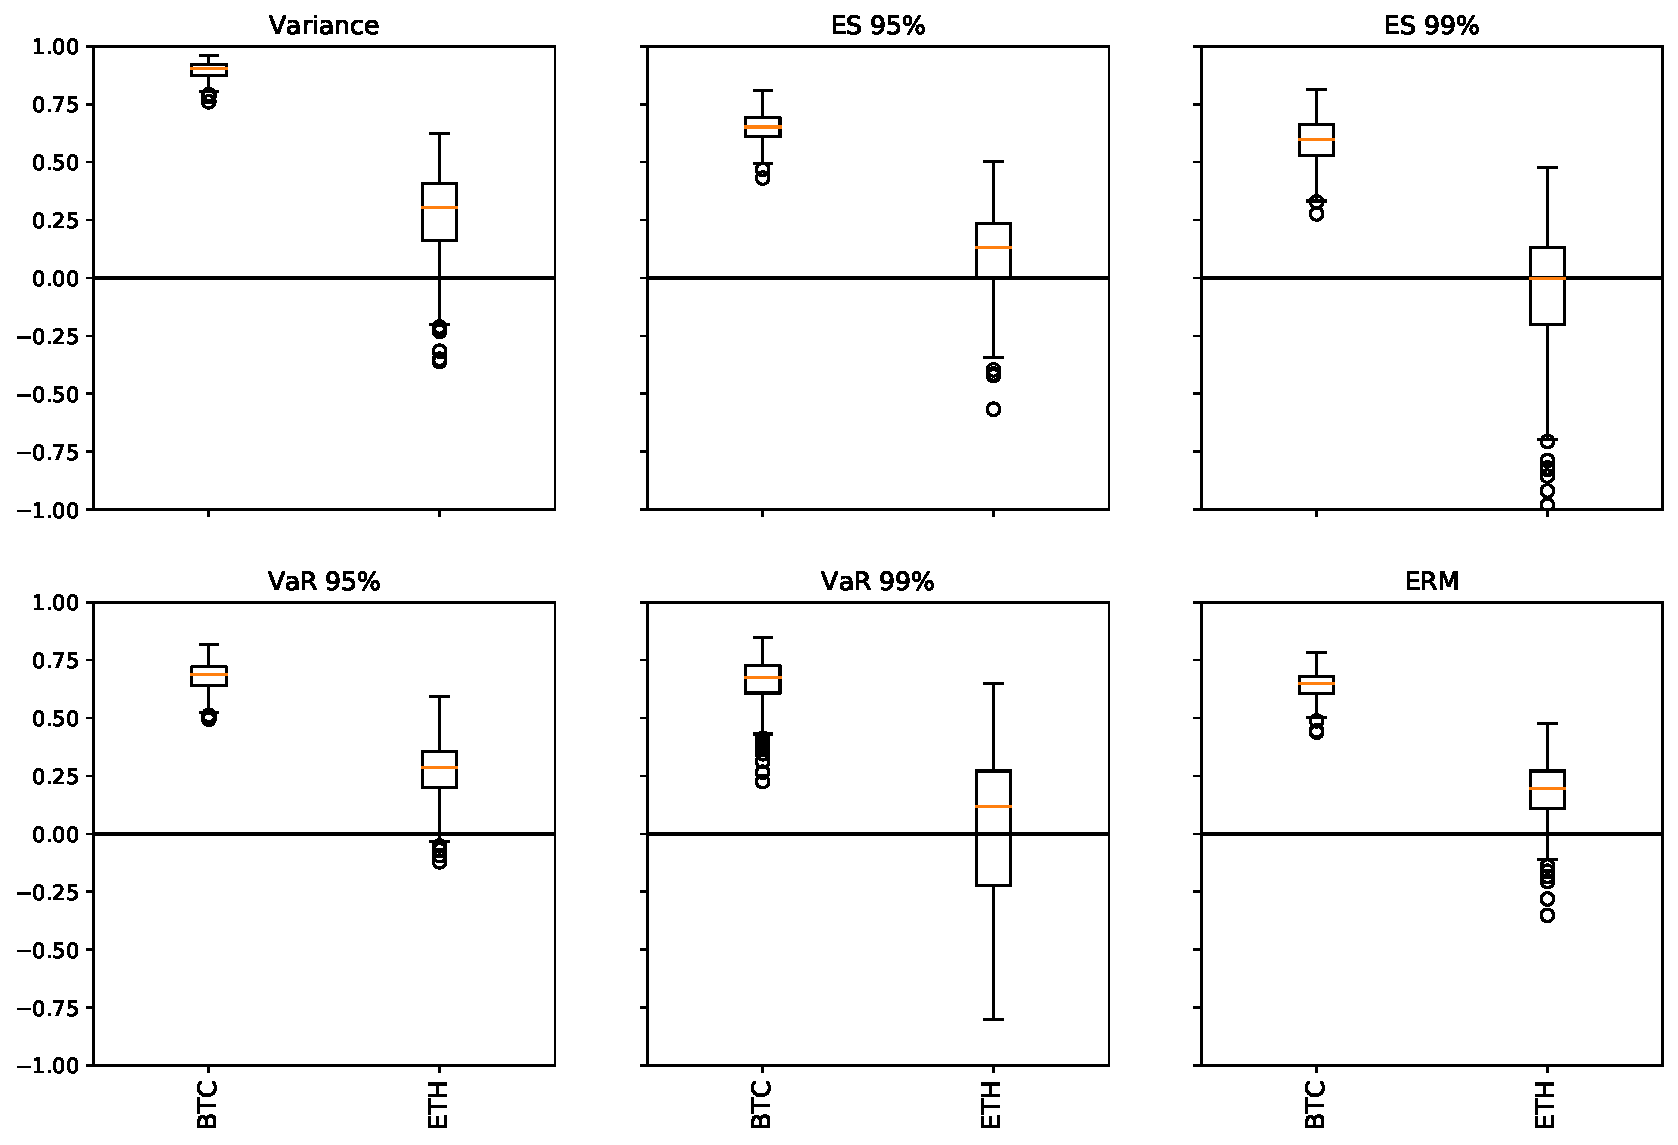
\includegraphics[width=\textwidth]{_pics/intraday_HE.pdf}
  \caption{Intraday HEs of BTC-BTCF and ETH-BTCF portfolio. The HEs of BTC-BTCF portfolios are significantly higher than $0$,
which suggests involving the BTCF in the portfolio can effectively reduce market risk.
The HEs of ETH-BTCF portfolios are lower than that of BTC-BTCF portfolios, and sometimes go below $0$.
We nullify the hedging ability of BTCF in this intraday ETH-BTCF setting.
  \href{https://github.com/QuantLet/Hedging-Cryptos-with-Bitcoin-Futures/blob/main/newToQuantlet/Pynotebooks/figures/intraday/figure 13.ipynb}{\includegraphics[height=\baselineskip]{_pics/qletlogo_tr.png}} }
\label{fig:HEboxplot_intraday}
\end{figure}

% \textit{Bootstrapped out-of-sample HEs}:
Figure \ref{fig:HEboxplot_intraday} presents the bootstrapped out-of-sample HEs. 
In general, the daily rebalancing results of BTC-BTCF carry over to the intraday rebalancing schedule;
The intraday rebalancing ETH-BTCF is different from its daily rebalancing counterpart.
The main difference between the intraday rebalancing and daily
rebalancing ETH-BTCF portfolio is that negative HEs appear in the
intraday results in all the risk measures we consider. 
This implies that hedgers cannot gain hedging potential from intraday dependence between BTC and ETH to hedge an ETH crypto position. 

Turning to BTC-BTCF, the HEs of BTC-BTCF are
significantly higher than zero across different risk measures,
suggesting that adding BTCF to a BTC portfolio can effectively reduce
the risk measured by selected measures.
Among risk measures, HE of variance is the highest, ranging between 72\% to 98\%, while the
  HE's other risk measures range between 25\% to 80\%.
Reducing variance being a well-achievable objective is
consistent with the findings of the daily rebalancing schedule.
On the other hand, the HEs of ES99\% and VaR99\% are relatively more dispersed and skewed to the left.
Both risk measures consider only 1\% of the data from the left for deciding the hedge ratio and computing the HEs.
Considering only a few data points naturally leads to a less reliable hedge ratio and lower consistency HEs.
Evidence also shows that ES99\% VaR99\% minimising portfolios have higher MSE and LSV.
This result is again consistent with the daily rebalancing setting.


\begin{figure}[t]
  \begin{center}
    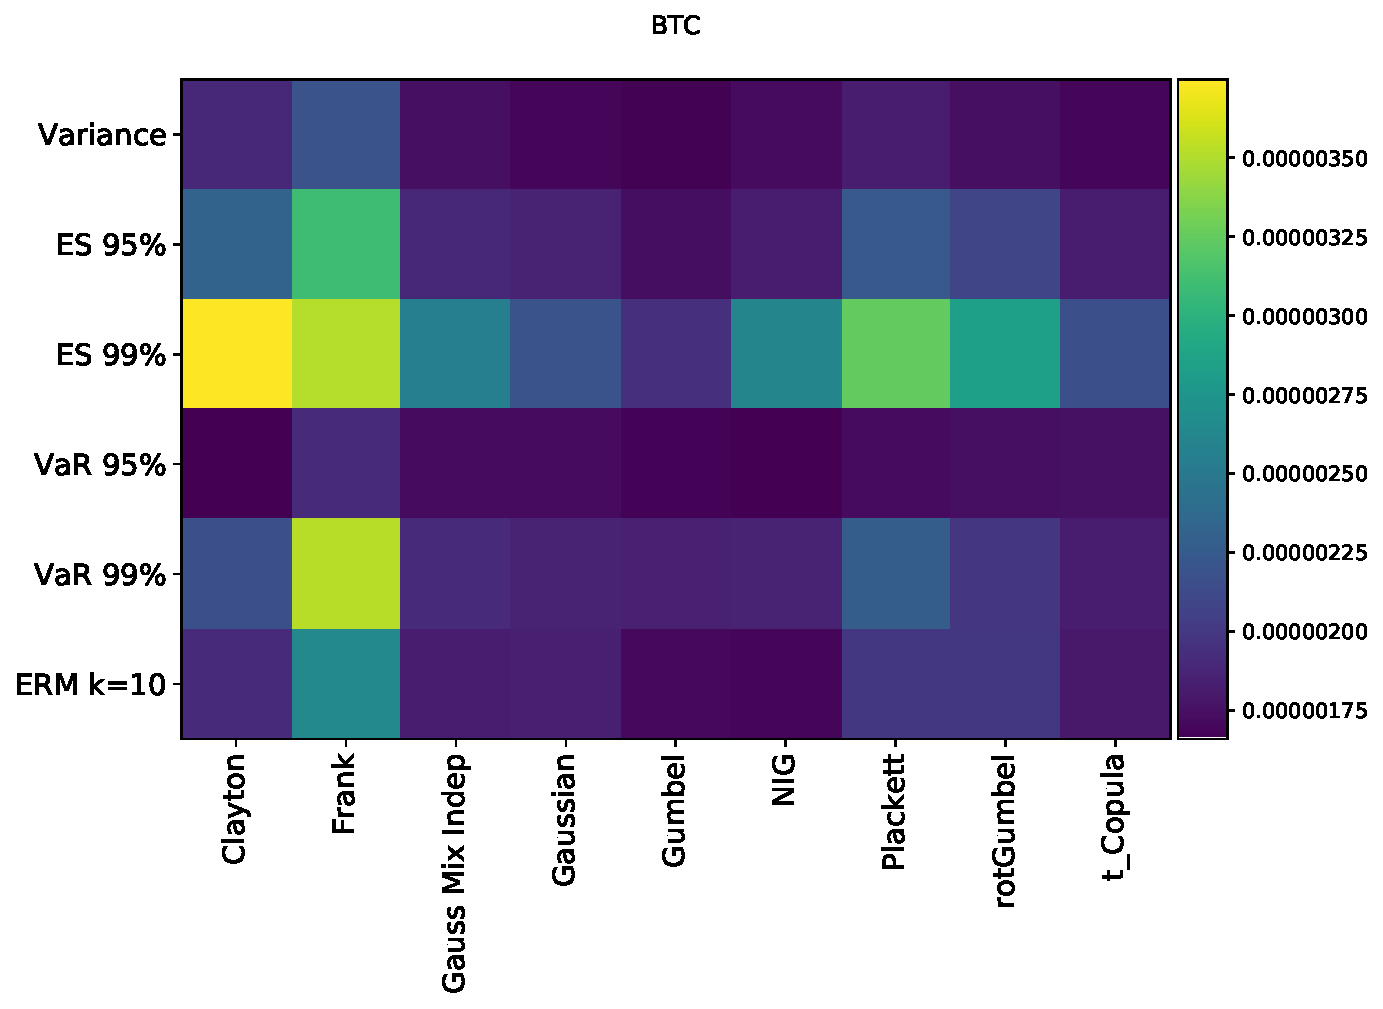
\includegraphics[width=.65\textwidth]{_pics/intraday_BTC_MSEs.pdf}
  \end{center}
  \caption{Intraday out-of-sample MSEs of the BTC-BTCF portfolio constructed by combinations of copula and risk measures.
    The Frank copula is again inferior. Minimising ES99\% results in higher MSEs disregard of which copula is in use.
  \href{https://github.com/QuantLet/Hedging-Cryptos-with-Bitcoin-Futures/blob/main/newToQuantlet/Pynotebooks/figures/intraday/gen_MSEs_LSVs.ipynb}{\includegraphics[height=\baselineskip]{_pics/qletlogo_tr.png}}
}
\label{fig:BTC_MSE}
\end{figure}

\begin{figure}[t]
  \begin{center}
    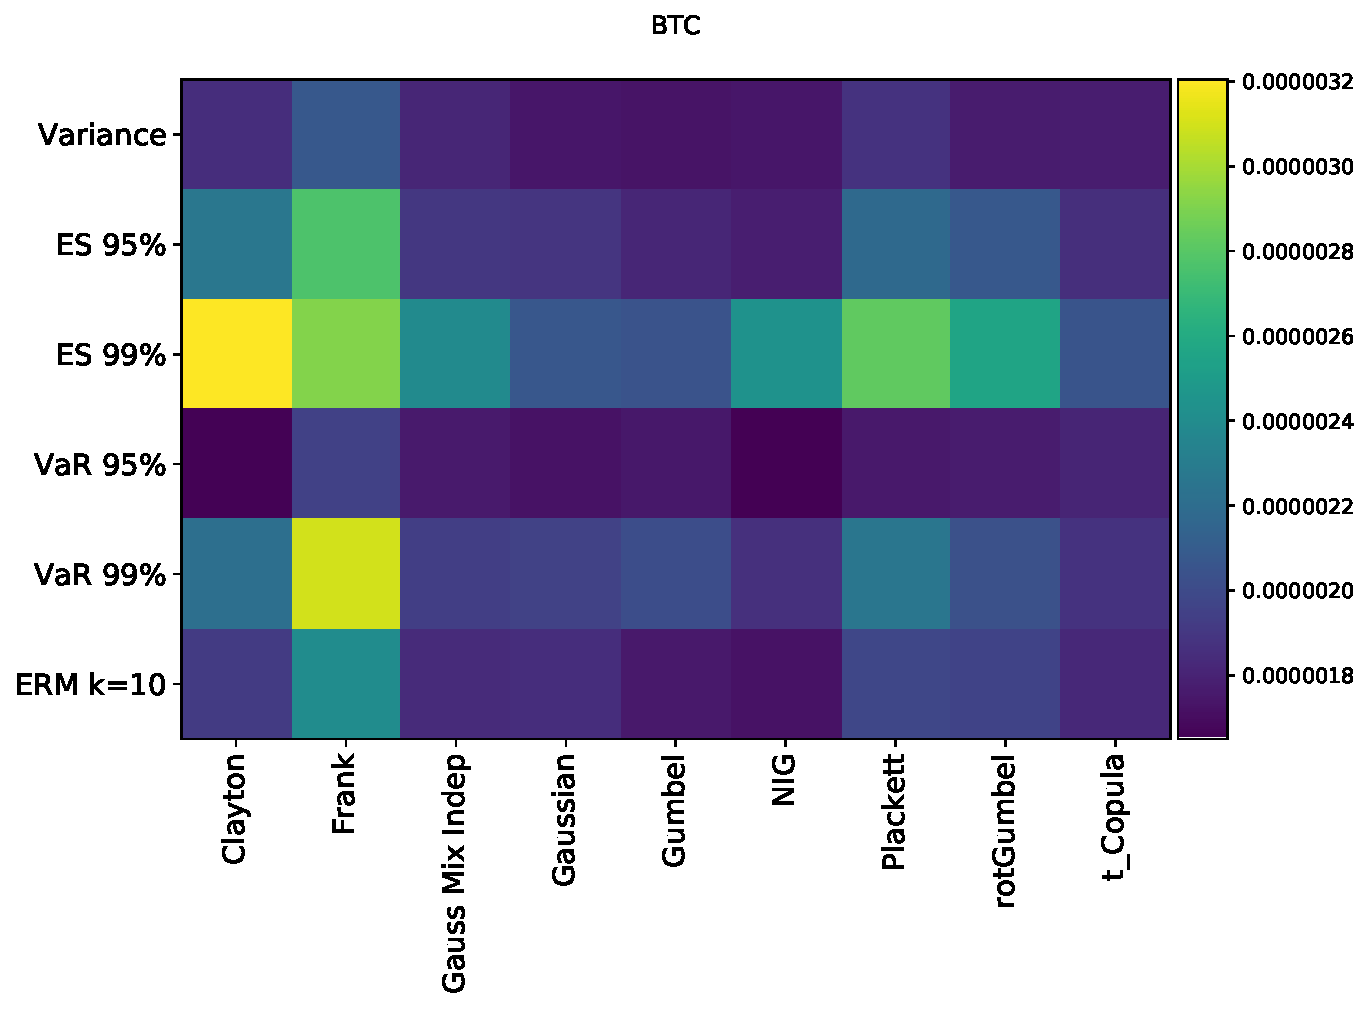
\includegraphics[width=.65\textwidth]{_pics/intraday_BTC_LSVs.pdf}
  \end{center}
  \caption{Intraday out-of-sample LSVs of the BTC-BTCF portfolio constructed by combinations of copula and ris minimization objectives.
    The Frank copula is again inferior. Minimising ES99\% results in higher MSEs disregard of which copula is in use.
  \href{https://github.com/QuantLet/Hedging-Cryptos-with-Bitcoin-Futures/blob/main/newToQuantlet/Pynotebooks/figures/intraday/gen_MSEs_LSVs.ipynb}{\includegraphics[height=\baselineskip]{_pics/qletlogo_tr.png}} }
\label{fig:BTC_LSV}
\end{figure}

Figures \ref{fig:BTC_MSE} and \ref{fig:BTC_LSV} report the
out-of-sample MSE and LSV of the BTC-BTCF when different copulae and
risk measures are in use. The MSEs and LSVs share similar patterns to that of the daily rebalancing
setting. 
Across various copulae, the BTC-BTCF portfolio that minimises VaR95\%
provides the lowest MSE and LSV. 
Portfolios that minimise variance and ERM with $k=10$ are close in MSEs and LSVs,
The MSEs and LSVs are slightly higher than that of VaR95\%, especially when Gumbel and NIG copulae
are in use to model the dependence. ES99\% generates the highest MSEs
and LSVs, regardless of the copula. 

Across various risk measures, Gumbel and NIG copulae perform
well in the resulting portfolios’ MSE and LSV, except for
ES99\%. 
The Frank copula performs worst, regardless of the risk measure. 
These results are consistent with the daily rebalancing setting and
conclusion drawn in \citet[p.667]{barbi2014copula}. 

\begin{table}[t]
  \centering
  \begin{tabularx}{\textwidth}{lYYYYY} \toprule
       Spot/ Copula & $t$ & Plackett & GMI & rotGumbel & NIG \\ \midrule
      \ \ \ BTC          & 60.00          & \phantom{0}1.11       & \phantom{0}3.33    & \phantom{0}8.89       & 26.67                  \\
      \ \ \ ETH          & 35.14          & \phantom{0}0.00       & 24.32              & 15.68                 & 24.86                   \\
  \bottomrule
  \end{tabularx}  
 \caption{Intraday copula selection results (shortened).
        The values are the percentage of counts of a copula chosen by the AIC procedure during the out-of-sample period.
        The table shows only the frequently chosen copula, i.e. $t$, Plackett, Gaussian Mix Independent (GMI), rotated Gumbel (rotGumbel), and
        Normal Inverse Gaussian factor copula (NIG).
        }
    \label{tab:copulasection_intraday}
\end{table}

Table \ref{tab:copulasection_intraday} shows the percentage of counts of a copula chosen by the AIC procedure over the out-of-sample period.

Most frequently chosen copulae are $t$-, Plackett, Gaussian Mix Independent, rotated Gumbel and NIG.
Similar to the result in the daily rebalancing schedule, most of the time the AIC procedure chooses t-Copula to model
the dependence structure of BTC-BTCF in the intraday setting.
For the rest of the time, the NIG copula is mainly chosen.
Rotated Gumbel, Gaussian Mix Independent, and Plackett are spontaneously chosen.
On the other hand, the intraday ETH-BTCF’s AIC selection result is very different from that of the daily rebalancing.
There are three copulae: $t$-, Gaussian Mix Independent, and NIG copula, that are closely chosen, instead of a single copula, rotated Gumbel copula, dominating the list in the daily rebalancing setting.
\end{document}